\documentclass[a4paper,12pt]{report}
\usepackage[utf8]{inputenc}
\usepackage[english]{babel}
\usepackage{fancybox}
\usepackage{fontenc}
\usepackage{a4wide}
\usepackage{graphicx}
\usepackage{placeins}
\usepackage{array}
\usepackage{adjustbox}
\usepackage{tabularx}
\usepackage[table,xcdraw]{xcolor}
\usepackage{wrapfig}
\usepackage{subcaption}
\usepackage{color, colortbl}
\definecolor{Gray}{gray}{0.9}
\definecolor{LightCyan}{rgb}{0.88,1,1}
\usepackage{longtable}
\usepackage{float}
\usepackage{lscape}
\usepackage{afterpage}
\usepackage{rotating}
\usepackage[nottoc,notlof,notlot]{tocbibind}
\usepackage{tocloft}
\usepackage{pdfpages}
\usepackage{ifthen}
\usepackage{ifpdf}
\usepackage{amsmath}
\usepackage{makeidx}
\usepackage{setspace}
\usepackage{epstopdf}
\usepackage{eurosym}
\usepackage[top=3cm, bottom=3cm, left=1.5cm, right=2cm]{geometry}
\usepackage{fancyhdr}
\usepackage{multirow,makecell}
\usepackage{blindtext}
\usepackage{caption}

% Toggle screenshots on/off (off => placeholders shown, no missing-file errors)
\newif\ifshowfigs
\showfigsfalse % set \showfigstrue to build with real screenshots

% Placeholder box for omitted images
\newcommand{\figplaceholder}[2][7cm]{%
  \fbox{%
    \parbox[c][#1][c]{0.92\textwidth}{\centering\small\itshape
      Screenshot omitted in the public report: #2}%
  }%
}

\graphicspath{{images/}{images_pfe/}{assets/}}
\newlength\figureheight
\newlength\figurewidth

\ifpdf
\usepackage[pdftex]{hyperref}
\else
\usepackage{hyperref}
\fi

\hypersetup{%
colorlinks=true,
linkcolor=black,
citecolor=black,
urlcolor=blue}

\setlength{\headheight}{16pt}
\pagestyle{fancy}
\setcellgapes{3pt}
\setlength{\parindent}{1.1cm}
\makegapedcells
\newcolumntype{R}[1]{>{\raggedleft\arraybackslash }b{#1}}
\newcolumntype{L}[1]{>{\raggedright\arraybackslash }b{#1}}
\newcolumntype{C}[1]{>{\centering\arraybackslash }b{#1}}
\renewcommand{\footrulewidth}{1pt}
\fancyfoot[C]{\textbf{\thepage}}
\fancyfoot[R]{Academic year 2024-2025}
\fancyfoot[L]{ENSIAS}
\fancyhead[L]{\nouppercase{\leftmark}}
\fancyhead[R]{\nouppercase{\rightmark}}
\pagenumbering{Roman}

\newcommand{\HRule}{\rule{\linewidth}{0.5mm}}

\begin{document}


% \documentclass[12pt]{report}
% \usepackage[utf8]{inputenc}
% \usepackage{graphicx}
% \usepackage[a4paper, total={6in, 9in}]{geometry}
% \usepackage[french]{babel}
% \usepackage{float}
% \usepackage{makecell}
% \usepackage{longtable}
% \renewcommand\cellgape{\Gape[4pt]}
% \setcounter{tocdepth}{4}
% \setcounter{secnumdepth}{4}
% \graphicspath{{images/}}
% \begin{document}

% \pagenumbering{gobble} % Supprimer la numérotation des pages




% Upper part of the page. The '~' is needed because only works if a paragraph has started.
\begin{titlepage}
\begin{center}

% Upper part of the page. The '~' is needed because only works if a paragraph has started.

\begin{minipage}{.2\textwidth}%

\includegraphics[width=.8\textwidth]{./assets/ensias.png}
 \end{minipage}%
 \hfill
 \begin{minipage}{.6\textwidth}%
 \centering
 
\includegraphics[width=0.2\textwidth]{./assets/DDS.png}
 \end{minipage}%
 \hfill
 \begin{minipage}{.2\textwidth}%
 
\includegraphics[width=\textwidth]{./assets/um5.png}
 \end{minipage} \\
 

\textsc{\large Ecole Nationale Supérieure d’Informatique et d’Analyse des Systèmes - RABAT \\ [0.2cm] Departement Web and Mobile Engineering}\\[0.8cm]

% Title
\begin{figure}[H]
    \begin{center}
    % \includegraphics[scale=0.4]{./1}
    \large Field : IDSIT
    \end{center}
\end{figure}

\vspace{1cm}

{\LARGE \bfseries Second Year Internship}

\vspace{2cm}

\textcolor{black}{\rule{\textwidth}{2pt}}

\vspace{0.5cm}
\begin{doublespace}
{\LARGE \bfseries Design and Implementation of a High-Availability Kubernetes Platform for Production-Grade Application Deployment}
\vspace{0.5cm}

\textcolor{black}{\rule{\textwidth}{2pt}}

\end{doublespace}
\vspace{2cm}


% Author and supervisor
\begin{minipage}{0.4\textwidth}
\begin{flushleft} \large
\emph{Realised by :}\\[0.4 cm]
TAMASNA \textsc{Anouar}\\
\end{flushleft}
\end{minipage}
\begin{minipage}{0.58\textwidth}
\begin{flushleft} \large
\emph { \hspace*{1.3cm}Jury :} \\[0.4 cm]
\hspace*{1.3cm} Pr. Khalid NAFIL \\ \hspace*{1.3cm} Pr. Karima MOUMANE

\end{flushleft}
\end{minipage}

\vspace{1.5cm}

% \begin{minipage}{0.4\textwidth}
% \begin{flushleft} \large
% \end{flushleft}
% \end{minipage}
% \begin{minipage}{0.58\textwidth}
% \begin{flushleft} \large
% \emph{ \hspace*{1.3cm} Encadrée par :}\\[0.4 cm] \hspace*{1.5cm} Pr. ZELLO Ahmed\\
% \end{flushleft}
% \end{minipage}

\vfill

% Bottom of the page
\vspace{1cm}
{\large Academic year 2024-2025}

\end{center}
\end{titlepage}

\begin{doublespace}
\newpage
\phantomsection
\addcontentsline{toc}{section}{Dedication}

\vspace*{1cm}
\begin{center}
    \textbf{\huge{Dedication}}
\end{center}
\vspace{1cm}

\large{
I dedicate this work to:\\
My mother, sources of tenderness and love, for her support throughout my school life.\\
My father, who has always supported me and did everything possible to help me.\\
my brothers and sisters, whom I love very much.\\
My extended family.\\
My dear friends and teachers.\\
All those who, from near or far, contributed to the development of this work.\\
May God grant them health and prosperity.}
\newpage
\phantomsection
\addcontentsline{toc}{section}{Thanks}

\vspace*{1cm}
\begin{center}
    \textbf{\huge{Acknowledgements}}
\end{center}

\vspace{1cm}
\large{
First of all, praise to God, Who guided me on the right path throughout the work and inspired me with the right steps and the right reflexes. Without His mercy, this work would not have come to fruition. 

I would like to extend our most sincere thanks to the members of the jury. Please accept in this work my sincere respect and deep gratitude. 

I would also like to thank Miss Nessrine LAFHAL very much, who, as supervisors of the project, were always attentive despite their impediments. their help was precious, as was the time they devoted to me. 

I do not forget my parents for their contributions, their support, and their patience. 

Finally, I would like to thank all my relatives and friends, who have always supported and encouraged me during the realization of this project. 

Thank you, everyone.
}

\end{doublespace}
\newpage
\phantomsection
\addcontentsline{toc}{section}{Summary}

\begin{center}
\vspace{9cm}
    \textbf{\huge{Summary}}
\end{center}

\begin{doublespace}
\vspace{1cm}
\large{
This report reflects the culmination of my work during my internship at Digital Data Service, where I successfully designed and deployed a high-availability Kubernetes infrastructure. The primary objective was to create a resilient and scalable environment capable of hosting production-grade applications while ensuring reliability, fault tolerance, and streamlined DevOps workflows.

The infrastructure leverages a modern cloud-native stack, including Rancher for cluster management, ArgoCD for GitOps-driven continuous delivery, and Cert-Manager for automated TLS certificate management. Core services such as Harbor (private container registry with security scanning), MinIO (object storage), Redis (high-availability caching), PostgreSQL HA (with pgAdmin), and Apache Tika were deployed and configured with persistent storage to guarantee data durability.

Ingress was managed through NGINX controller, enabling secure external access via custom domains. The solution was designed with automation, scalability, and maintainability in mind, supporting dynamic workloads and reducing operational overhead.

Throughout the project, I focused on ensuring high availability, performance optimization, and security, while integrating DevOps best practices to meet the requirements of both developers and system administrators.

\textbf{Key-words:} Kubernetes HA, GitOps / ArgoCD, Rancher, CI/CD, DevOps
}


\newpage
\phantomsection
\addcontentsline{toc}{section}{Résumé}

\begin{center}
\vspace{9cm}
    \textbf{\huge{Résumé}}
\end{center}

\begin{doublespace}
\vspace{1cm}
\large{
Ce rapport reflète l’aboutissement de mon travail réalisé durant mon stage au sein de Digital Data Service, où j’ai conçu et déployé une infrastructure Kubernetes haute disponibilité. L’objectif principal était de mettre en place un environnement résilient et évolutif, capable d’héberger des applications de niveau production tout en garantissant fiabilité, tolérance aux pannes et automatisation des workflows DevOps.

L’infrastructure s’appuie sur un écosystème moderne cloud-native, incluant Rancher pour la gestion des clusters, ArgoCD pour le déploiement continu basé sur GitOps, et Cert-Manager pour la gestion automatisée des certificats TLS. Des services clés tels que Harbor (registre privé de conteneurs avec analyse de sécurité), MinIO (stockage objet), Redis (cache haute disponibilité), PostgreSQL HA (avec pgAdmin), et Apache Tika ont été déployés et configurés avec un stockage persistant afin d’assurer la durabilité des données.

L’accès externe a été géré via les contrôleur NGINX , permettant une exposition sécurisée des applications à travers des domaines personnalisés. La solution a été conçue dans une optique d’automatisation, de scalabilité et de maintenabilité, tout en réduisant la charge opérationnelle.

Tout au long du projet, je me suis concentré sur la garantie de la haute disponibilité, l’optimisation des performances et la sécurité, en intégrant les bonnes pratiques DevOps afin de répondre aux besoins des développeurs.
}
\end{doublespace}
\end{doublespace}
\newpage
\phantomsection
\addcontentsline{toc}{section}{Abbreviations List}

\begin{center}
\vspace{9cm}
    \textbf{\huge{Abbreviations List}}
\end{center}
\vspace{1cm}

\begin{doublespace}
\begin{center}
\begin{tabular}{|l|l|}
  \hline
  Abbreviation &  Designation \\
  \hline
  HA & High Availability \\
  \hline
  CI/CD & Continuous Integration / Continuous Deployment \\
  \hline
  PVC & Persistent Volume Claim \\
  \hline
  DNS & Domain Name System \\
  \hline
  GitOps & Git-based Operations \\
  \hline
  HTTP & Hypertext Transfer Protocol                   \\
  \hline
  HTTPS & Hypertext Transfer Protocol Secured \\
  \hline
\end{tabular}
\end{center}
\end{doublespace}

\newpage
\renewcommand{\contentsname}{Table Of Contents}
\setcounter{tocdepth}{3}
\tableofcontents

\newpage
\listoffigures
\newpage

\cleardoublepage
% \phantomsection
% \addcontentsline{toc}{chapter}{\listfigurename}

\pagenumbering{arabic} % Commencer la numérotation des pages à partir de la 10ème page en chiffres arabes
%\setcounter{page}{10}

% \cleardoublepage
\renewcommand{\headrulewidth}{1pt}
\fancyhead[R]{\textbf{General Introduction}}
\fancyhead[L]{\hspace*{4cm}}

\phantomsection
\addcontentsline{toc}{section}{General Introduction}
\begin{center}
\vspace{9cm}
    \textbf{\huge{General Introduction}}
\end{center}
\begin{doublespace}
\vspace{1cm}
\hspace{1cm}In recent years, the adoption of \textbf{cloud-native technologies} and \textbf{Kubernetes orchestration} has transformed the way organizations deploy and manage applications.\\
Ensuring \textbf{high availability, scalability, and fault tolerance} has become essential for production-grade workloads, particularly for businesses that rely on continuous service delivery and resilient infrastructure.\\

Our internship took place at \textbf{Digital Data Service}, where we worked on designing and deploying a \textbf{high-availability Kubernetes infrastructure}.\\
This environment supports the deployment of multiple production-grade services, including \textbf{ArgoCD} for GitOps-driven continuous delivery, \textbf{Rancher} for cluster management, \textbf{Harbor} as a private container registry, \textbf{MinIO} for object storage, \textbf{Redis} for caching, \textbf{PostgreSQL HA} for relational data management, \textbf{Apache Tika} for document processing, and two key company services, \textbf{NeuroTalk} and \textbf{HealthCore}.\\
We also implemented \textbf{NGINX Ingress controllers} for secure external access and configured \textbf{persistent storage} for all critical services to ensure \textbf{data durability}.\\

The presentation of this report is structured into \textbf{four chapters}.\\
The first chapter presents the internship environment, outlines the challenges addressed, introduces the proposed solution, and details the methodology followed.\\
The second chapter focuses on the \textbf{analysis of system components}, infrastructure requirements, and best practices for high availability and security, including the staging and deployment of \textbf{NeuroTalk} and \textbf{HealthCore}.\\
The third chapter covers the \textbf{design and architecture}, with detailed diagrams of the Kubernetes cluster, services, and networking setup.\\
Finally, the fourth chapter presents the \textbf{deployment and operational procedures}, including configuration of persistent volumes, GitOps pipelines, monitoring tools, and deployment strategies for \textbf{NeuroTalk} and \textbf{HealthCore}.\\

It is important to note that this project involved \textbf{building a resilient and scalable platform from scratch}, automating deployments, ensuring \textbf{high availability and fault tolerance}, and integrating \textbf{security and monitoring solutions} to meet production standards while minimizing operational overhead, while also successfully staging and supporting \textbf{NeuroTalk} and \textbf{HealthCore}.\\
\end{doublespace}

\newpage
\renewcommand{\headrulewidth}{1pt}
\fancyhead[L]{\textbf{Chapter I: General Project Context}}
\fancyhead[R]{\hspace*{4cm}}

\setcounter{chapter}{1}
\begin{doublespace}
\phantomsection
\addcontentsline{toc}{chapter}{Chapter I : Work Context}
\vspace*{10cm}
\centering
\textbf{ \huge Chapter I \\ [1 cm] General Project Context}
\end{doublespace} 
\newpage 
\begin{doublespace}

\end{doublespace}

\fancyhead[R]{\nouppercase{\rightmark}}
\section*{Introduction}
\begin{doublespace}

\hspace{1cm}In this first chapter, we delve into the context of our project, focused on the development and enhancement of a \textbf{high-availability Kubernetes infrastructure}.\\
\hspace{1cm}Our initiative involves deploying a resilient platform with multiple production-grade services, including \textbf{ArgoCD}, \textbf{Rancher}, \textbf{Harbor}, \textbf{MinIO}, \textbf{Redis}, \textbf{PostgreSQL HA}, \textbf{Apache Tika}, and two key company services, \textbf{NeuroTalk} and \textbf{HealthCore}.\\
\hspace{1cm}We also implemented secure \textbf{NGINX Ingress controllers} and configured persistent storage for all critical services to ensure \textbf{data durability}.\\
\hspace{1cm}This work takes place in a dynamic professional environment at \textbf{Digital Data Service}, a company specializing in IT infrastructure and cloud-native solutions.\\
\hspace{1cm}Our goals are to ensure \textbf{high availability, scalability, and fault tolerance} of deployed applications, streamline management of the infrastructure, implement robust monitoring and security practices, and provide reliable staging and deployment for key company services like \textbf{NeuroTalk} and \textbf{HealthCore}.\\
\hspace{1cm}This introduction lays the essential foundations for understanding the scope and objectives of our project.
\end{doublespace}


\section{Internship Environment}
\begin{doublespace} ~\\[0cm]


\includegraphics[width=0.2\textwidth]{./assets/DDS.png}~\\[2cm]

 \textbf{Digital Data Service} is a startup committed to supporting businesses in their digital journey. Through a diverse range of digital services tailored to the local context, we facilitate their technological transition in a strategic, agile, and customized manner.[1]
\begin{figure}[H]
    \centering
    \begin{adjustbox}{max width=\textwidth}
    \begin{tabular}{|p{0.33\textwidth}|p{0.65\textwidth}|}
      \hline
      Company Name & Digital Data Service \\
      \hline
      Headquarters & Casablanca, Morocco \\
      \hline
      represented by & Mr. Anas TAHA \\
      \hline
      Staff & 10 employees and 8 interns \\
      \hline
      Website & https://www.digitaldataservices.ma \\
      \hline
      Email & contact@digitaldataservices.ma \\
      \hline
      Phone & +212 777-077986 \\
      \hline
    \end{tabular}
    \end{adjustbox}
    \caption{Digital Data Service — Company Profile}
\end{figure}

\end{doublespace}


\section{Project Presentation}
\begin{doublespace}

\subsection{Problem Statement}
\hspace{1cm}In modern IT environments, organizations face major challenges when deploying and managing complex infrastructures. 
Companies need to ensure \textbf{high availability, scalability, and fault tolerance} for their mission-critical applications, while also guaranteeing secure access, data durability, and efficient deployment pipelines. \\
Traditional infrastructures often suffer from issues such as downtime, limited scalability, inefficient communication between services, security vulnerabilities, and the absence of centralized monitoring and management solutions. \\
Moreover, deploying multiple production-grade services like \textbf{ArgoCD}, \textbf{Rancher}, \textbf{Harbor}, \textbf{MinIO}, \textbf{Redis}, and \textbf{PostgreSQL HA}, in addition to core company services such as \textbf{NeuroTalk} and \textbf{HealthCore}, introduces significant complexity that requires a robust, automated, and secure Kubernetes-based platform.

\subsection{Proposed Solutions}
\hspace{1cm}Our project addresses these challenges by designing and deploying a fully integrated \textbf{high-availability Kubernetes infrastructure} that ensures resilience, scalability, and operational efficiency. 
The key solutions we implemented include: \\

\textbf{-} \textit{Modern and user-friendly platform management:} We integrated \textbf{Rancher} for centralized cluster management, providing a clean and intuitive interface to handle multiple Kubernetes clusters securely and efficiently. \\

\textbf{-} \textit{Continuous delivery and automation:} Using \textbf{ArgoCD}, we implemented GitOps practices, enabling automated, reliable, and version-controlled deployments for all applications and services. \\

\textbf{-} \textit{Secure storage and artifact management:} We deployed \textbf{Harbor} as a private container registry and configured persistent volumes for all critical services such as \textbf{MinIO} and \textbf{PostgreSQL HA}, ensuring data durability and compliance with enterprise standards. \\

\textbf{-} \textit{High availability and scalability:} The platform was built with multiple replicas, fault-tolerant deployments, and an \textbf{NGINX Ingress controller} for secure load balancing and traffic routing across services. \\

\textbf{-} \textit{Monitoring, communication, and transparency:} We established a robust monitoring and logging stack to track service health and performance. Additionally, our approach allows clear visibility over deployed applications, ensuring transparency for both system administrators and developers. \\

\textbf{-} \textit{End-to-end integration for company services:} NeuroTalk and HealthCore, as core business applications, were deployed on the platform with complete support for CI/CD pipelines, persistence, and scalability, enabling seamless operations and reliable staging environments. \\

Through these solutions, our project provides a secure, highly available, and scalable infrastructure that addresses the critical needs of modern enterprises while laying the foundation for future growth and innovation.

\end{doublespace}

\section{Project Planning (Gantt Chart):}
\begin{doublespace}
\subsection{Gantt Chart}
\hspace{1cm}Our project was managed by following a chronological breakdown into phases, which specify what must be done (tasks) and by whom (resources). To represent this distribution, we use a Gantt Chart, a type of bar chart that illustrates a series of tasks over a given period of time. \\

This chart provides a clear overview of the activities carried out within the project, including their start and end dates, and constitutes a visual representation of the project timeline. \\

In our case, the Gantt Chart highlights the different stages of deployment and testing in the Kubernetes environment (K3s cluster). It includes tasks such as setting up the cluster infrastructure, configuring networking and Ingress (without Traefik), ensuring persistence with MinIO, and staging two company services, namely \textbf{NeuroTalk} and \textbf{HeathCore}, before moving to production. \\

Here is an example of our \textbf{Gantt Chart} that illustrates the main milestones and phases of our project: \\
\begin{figure}[H]
    \centering
    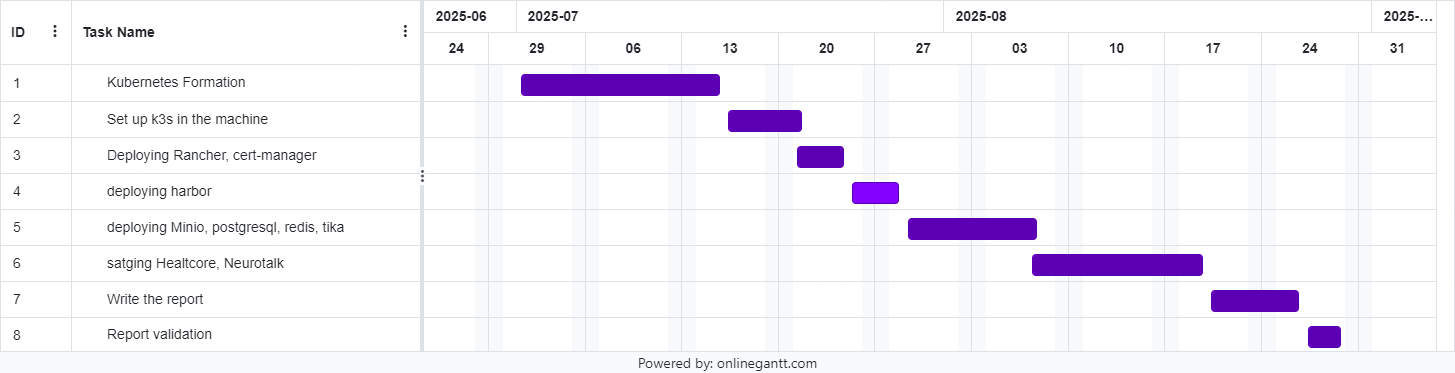
\includegraphics[width=\textwidth]{./assets/DDSGaint.png}
    \caption{GANTT chart}
\end{figure}
\end{doublespace}

\section{Conclusion}
\begin{doublespace}
\hspace{1cm}This first chapter immersed us in the general context of our project, highlighting the working environment within \textbf{Digital Data Service (DDS)}. We presented the motivations behind our initiative, as well as the challenges related to infrastructure deployment, service management, and the need for a reliable and scalable environment. \\

We also introduced the core objectives of our work, including the deployment of a Kubernetes (K3s) cluster, the configuration of networking and persistence services, and the staging of two key company platforms: \textbf{NeuroTalk} and \textbf{HeathCore}. These steps constitute the foundation for a secure, efficient, and production-ready system. \\

In the next chapter, we will address a crucial phase: the \textbf{requirements analysis}. We will explore in depth the specific needs of users and stakeholders, both from a technical and business perspective. This stage is essential to design a solution that meets all expectations and requirements. \\

A detailed analysis of these needs will establish a solid foundation for the subsequent development and optimization of our project. Let us now move to the next chapter, where we will dive into this comprehensive study of requirements. \\
\end{doublespace}

\renewcommand{\headrulewidth}{1pt}
\fancyhead[L]{\textbf{Chapter II: Needs Analysis}}
\fancyhead[R]{\hspace*{4cm}}

\setcounter{chapter}{2}
\begin{doublespace}
\phantomsection
\addcontentsline{toc}{chapter}{Chapter II: Needs Analysis}
\vspace*{10cm}
\centering
\textbf{ \huge Chapter II \\ [1 cm] Needs Analysis}
\end{doublespace}
\setcounter{section}{0}
\newpage
\fancyhead[R]{\nouppercase{\rightmark}}
\begin{doublespace}
\section{Introduction}
\hspace{1cm}The company operates in the field of digital data services and requires robust, reliable, and secure infrastructure to support its growing activities. The goal of this project is to design and deploy a solution that ensures high availability (HA), scalability, and optimized resource management for production workloads. This approach guarantees continuity of services, resilience against failures, and the ability to handle increasing demand efficiently.

\section{Needs Identification}
\hspace{1cm}In the context of digital data services, the focus is not on end-users but rather on the infrastructure and operational requirements. The following needs have been identified as critical for the company’s environment: \\

\textbf{High Availability (HA):}  
The system must be resilient and capable of running without service interruption, even in the case of node or component failure. This includes load balancing, failover mechanisms, and redundancy across services. \\

\textbf{Scalability:}  
The infrastructure should be able to scale both vertically (adding more resources to a node) and horizontally (adding more nodes to the cluster) to support increasing workloads as the company grows. \\

\textbf{Monitoring and Observability:}  
The company needs full visibility into system health, performance, and availability. This requires setting up centralized logging, metrics collection, and alerting systems to quickly detect and resolve incidents. \\

\textbf{Automation and CD Pipelines:}  
To streamline deployments and reduce manual intervention, infrastructure and application delivery must rely on automation tools and CD pipelines. This will ensure consistency, faster releases, and reduced risk of configuration errors. \\

\textbf{Security and Compliance:}  
Given the sensitive nature of digital data services, the deployment must include strong security practices such as secret management, encrypted communication, controlled access, and compliance with industry standards. \\

\textbf{Cost Optimization:}  
The infrastructure should balance performance and reliability with cost-effectiveness. This includes the use of containerization, resource quotas, and autoscaling policies to prevent over-provisioning. \\

Together, these requirements will guide the design and deployment of an infrastructure that meets the company’s operational, business, and security objectives.
\end{doublespace}

\section{Functional Requirements Specification:}
\hspace{1cm}The infrastructure will be designed to provide the following functionalities: \\

\textbf{High Availability Management:}  
The deployment must guarantee continuous service availability through redundancy, clustering, and automated failover mechanisms. Even in the event of node or component failure, the system should remain fully operational. \\

\textbf{Scalability and Elasticity:}  
The solution should allow both vertical and horizontal scaling to handle increasing workloads. Autoscaling mechanisms will be implemented to allocate resources dynamically, ensuring efficiency without over-provisioning. \\

\textbf{Monitoring and Observability:}  
Centralized logging, monitoring, and alerting will be deployed to track system health, performance, and availability. This includes dashboards to visualize resource utilization, error rates, and real-time service status. \\

\textbf{Automation and CD Pipelines:}  
Deployment, updates, and configuration management must be automated through DevOps pipelines. This ensures consistency across environments, reduces human error, and accelerates release cycles. \\

\textbf{Disaster Recovery and Backup:}  
The infrastructure will include automated backups, recovery strategies, and geographic redundancy to minimize downtime and data loss in case of major incidents. \\

\textbf{Security and Access Control:}  
The solution must ensure secure communication, identity management, and secret storage. Policies such as role-based access control (RBAC), TLS encryption, and compliance standards will be enforced. \\

\textbf{Resource and Cost Management:}  
Dashboards and tools will allow tracking of infrastructure usage and costs. Autoscaling and quota management will ensure optimized resource allocation. \\


\section{Non-Functional Requirements Specification:}
To ensure smooth operation and user satisfaction, several non-functional constraints must be taken into account during the design and implementation of the project: \\

\begin{itemize}
    \item \textbf{Performance and Reliability:} \\  
    The system must be responsive and highly available, maintaining reliable performance under varying workloads.

    \item \textbf{Scalability:} \\  
    The solution should handle future growth seamlessly by scaling horizontally with additional nodes and services.

    \item \textbf{Security:} \\  
    Data integrity and confidentiality must be guaranteed. The system should include encryption, intrusion detection, secure APIs, and compliance with security standards.

    \item \textbf{Maintainability:} \\  
    The infrastructure code (Infrastructure-as-Code) must be well-structured, modular, and documented to facilitate future updates and enhancements.

    \item \textbf{Compatibility:} \\  
    The deployment must be compatible with multi-cloud and hybrid environments. It should support containerized workloads and be portable across different environments.

    \item \textbf{Monitoring and Transparency:} \\  
    The system must provide visibility into all layers of the infrastructure, with real-time metrics and logs accessible to the DevOps team.

    \item \textbf{Ease of Use:} \\  
    Interfaces such as dashboards and management consoles must be intuitive and easy for administrators to operate.
\end{itemize}


\section{Conclusion}
\begin{doublespace}
\hspace{1cm}This second chapter allowed us to explore in detail the specific needs of the company, focusing on the deployment of a high availability and scalable infrastructure. We identified the main challenges and proposed solutions addressing reliability, performance, and security requirements. \\

By concentrating on the needs analysis, this phase represents a crucial foundation for the design of a robust and resilient DevOps architecture. The detailed analysis conducted here provides a solid basis for the next phase of the project. \\

In the next chapter, we will move on to analysis and design, including architectural modeling and deployment planning. These steps will allow us to translate the identified requirements into concrete technical solutions. 
\end{doublespace}
\newpage

\renewcommand{\headrulewidth}{1pt}
\fancyhead[L]{\textbf{Chapter III: Analysis and Design}}
\fancyhead[R]{\hspace*{4cm}}

\setcounter{chapter}{3}
\begin{doublespace}
\phantomsection
\addcontentsline{toc}{chapter}{Chapter III: Analysis and Design}
\vspace*{10cm}
\centering
\textbf{ \huge Chapter III \\ [1 cm] Analysis and Design}
\end{doublespace}
\setcounter{section}{0}
\newpage
\fancyhead[R]{\nouppercase{\rightmark}}
\begin{doublespace}
\section*{Introduction}
\hspace{1cm}The creation of a robust and highly available platform must be preceded by a thorough analysis and design phase. This ensures that the development process aligns perfectly with the project's requirements.

In this chapter, we'll focus on the architectural design of our platform. We'll present general diagrams that model and describe the desired operation of our Kubernetes infrastructure. Two conceptual perspectives will be described: the first gives an overview of the platform's core components, and the second provides a detailed view of the application deployment workflows.

\section{Infrastructure Component Diagram}
\hspace{1cm}The first step in our design process was to model the relationships between the core services of our Kubernetes cluster. This component diagram illustrates how \textbf{Harbor}, \textbf{Rancher}, \textbf{Ingress}, \textbf{Cert-Manager}, and other key elements interact to form a coherent and functional system.

\begin{figure}[H]
\centering
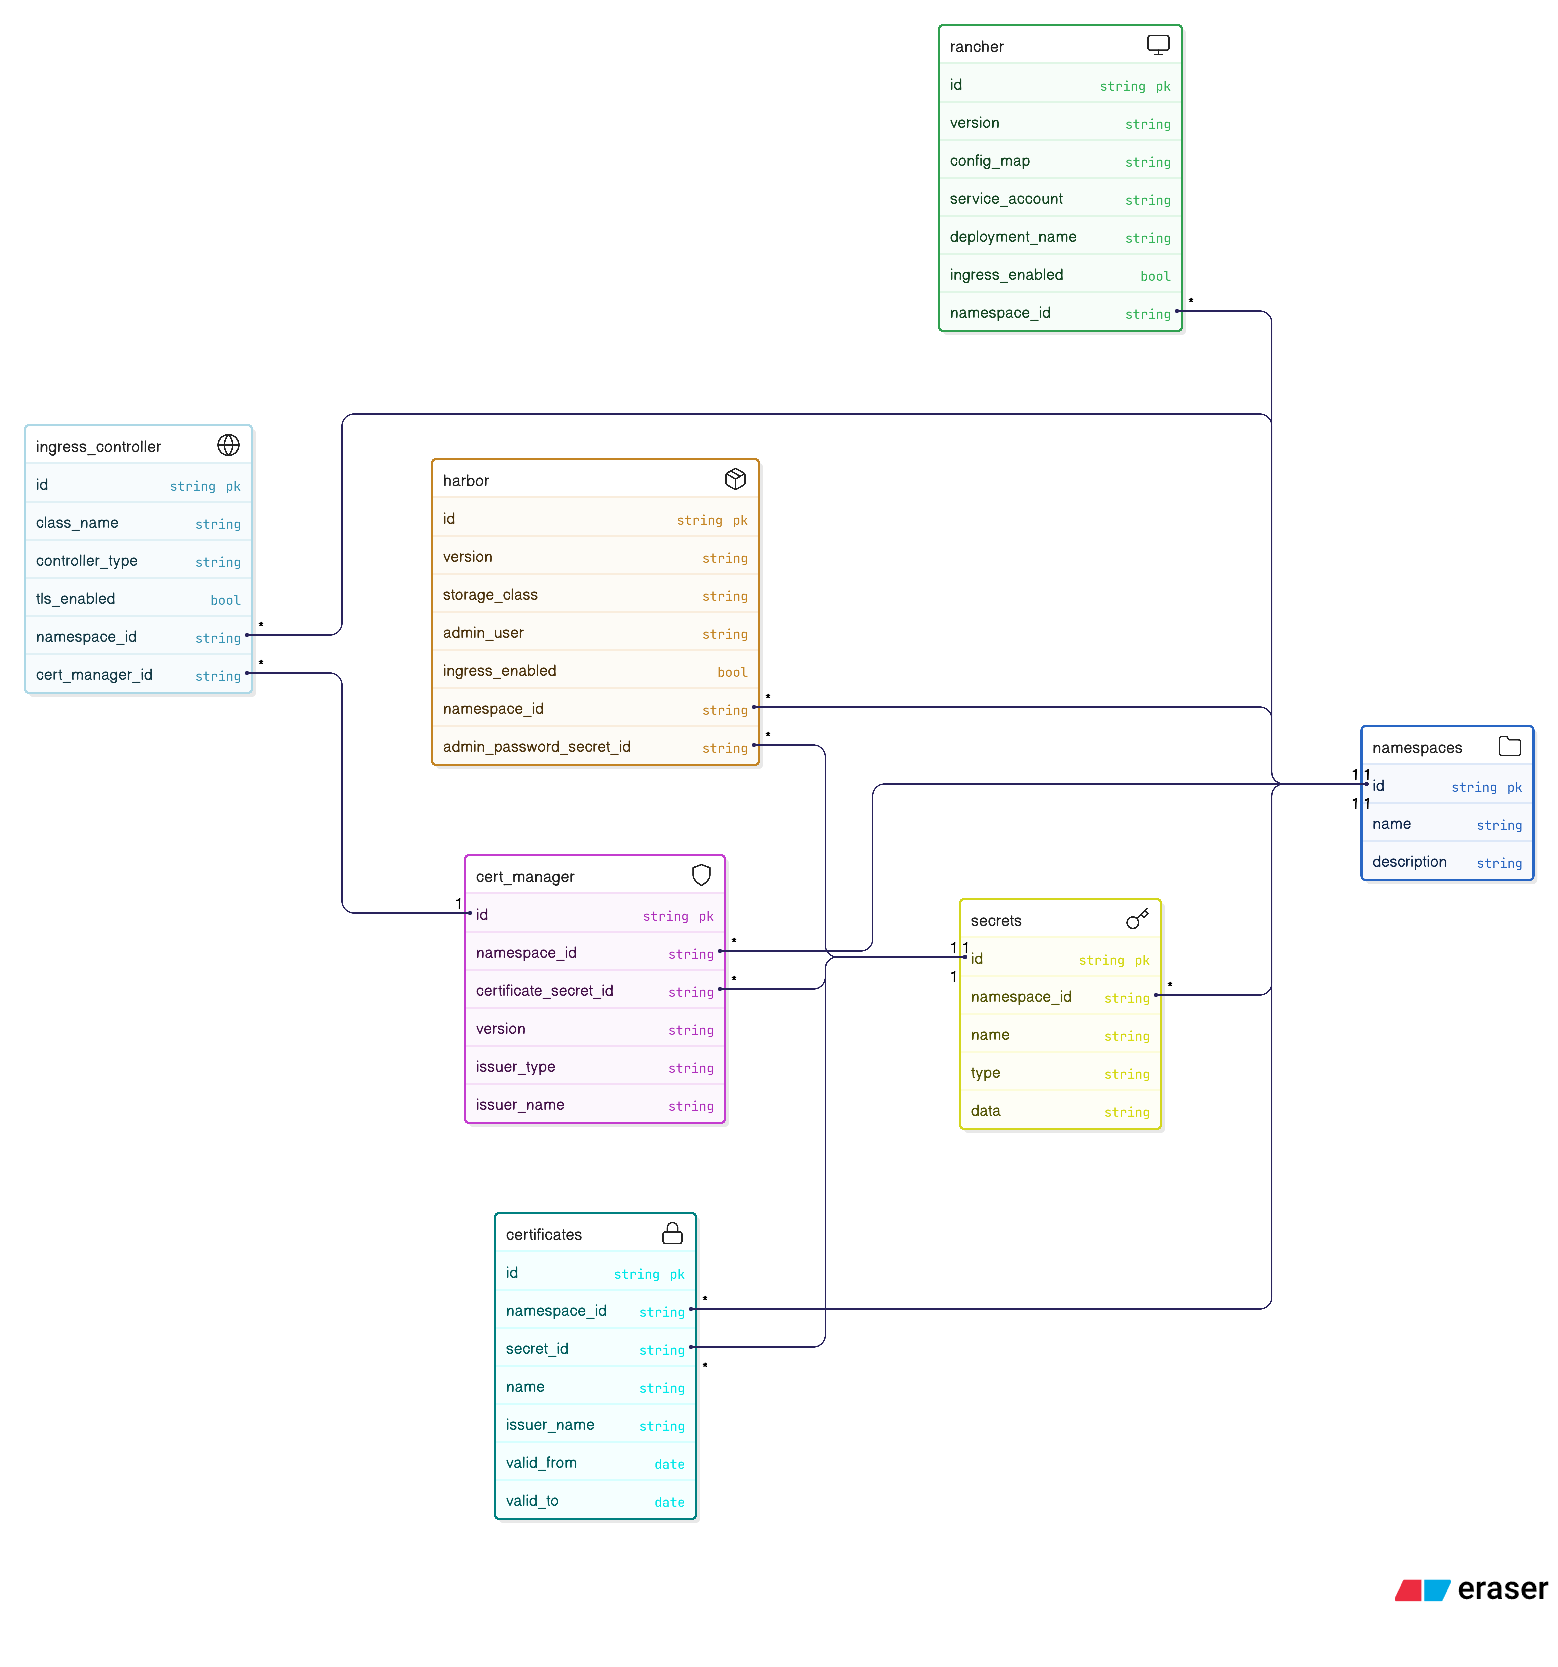
\includegraphics[width=\textwidth]{./assets/Harbor,Rancher,onecluster.png}
\caption{Infrastructure Component Diagram}
\end{figure}

As shown in the diagram, \textbf{Rancher} acts as the central management plane for our cluster, providing a user-friendly interface to manage multiple environments and namespaces. The \textbf{Ingress Controller} manages external access and routing, working in tandem with \textbf{Cert-Manager} to automatically provision and renew TLS certificates for secure communication. \textbf{Harbor} is our private container registry, ensuring that all our application images are stored securely and are accessible by the cluster. These services all depend on \textbf{Secrets} and \textbf{Namespaces} to handle sensitive information and logically isolate resources within the cluster.

This high-level view helps us understand the logical dependencies and ensures a robust foundation for the entire infrastructure.

\section{Application Deployment Workflows}
\hspace{1cm}To demonstrate the platform's capabilities, we designed a \textbf{Continuous Integration/Continuous Deployment (CD)} pipeline for two of the company's core applications: \textbf{HealthCore} and \textbf{NeuroTalk}. These workflow diagrams illustrate the end-to-end process, from code commit to application deployment, using a \textbf{GitOps} approach.

\subsection{HealthCore Workflow}
\hspace{1cm}The HealthCore workflow diagram details how the application is built, deployed, and managed. The process begins in the \textbf{CD Pipeline}, where code changes in \textbf{GitLab} trigger a CI job. This job builds the application image and pushes it to our private registry, \textbf{Harbor}, and updates the deployment manifests in the Git repository.

\begin{figure}[H]
\centering
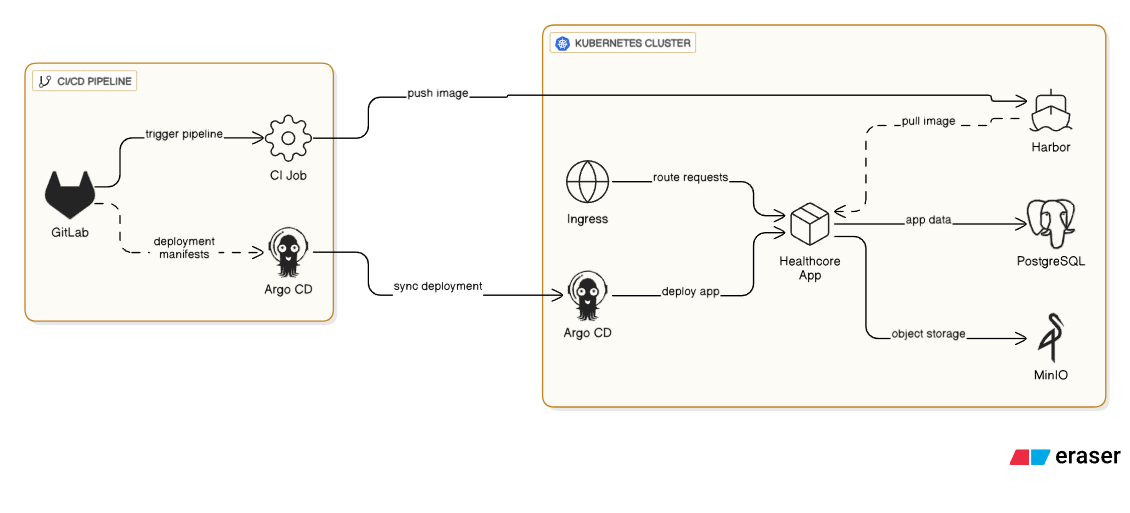
\includegraphics[width=\textwidth]{./assets/healthcore flow.png}
\caption{HealthCore Workflow Diagram}
\end{figure}

From there, \textbf{ArgoCD} takes over. As a GitOps tool, it constantly monitors the Git repository for changes. When a new commit with updated deployment manifests is found, ArgoCD automatically synchronizes the changes with the \textbf{Kubernetes Cluster}, pulling the new image from Harbor and deploying the \textbf{HealthCore App}. External traffic is then routed to the application through the \textbf{Ingress} controller. The application itself relies on persistent storage, connecting to a \textbf{PostgreSQL} database for application data and \textbf{MinIO} for object storage.

\subsection{NeuroTalk Workflow}
\hspace{1cm}The NeuroTalk workflow is similar but includes more complex application services to handle specific tasks.

\begin{figure}[H]
\centering
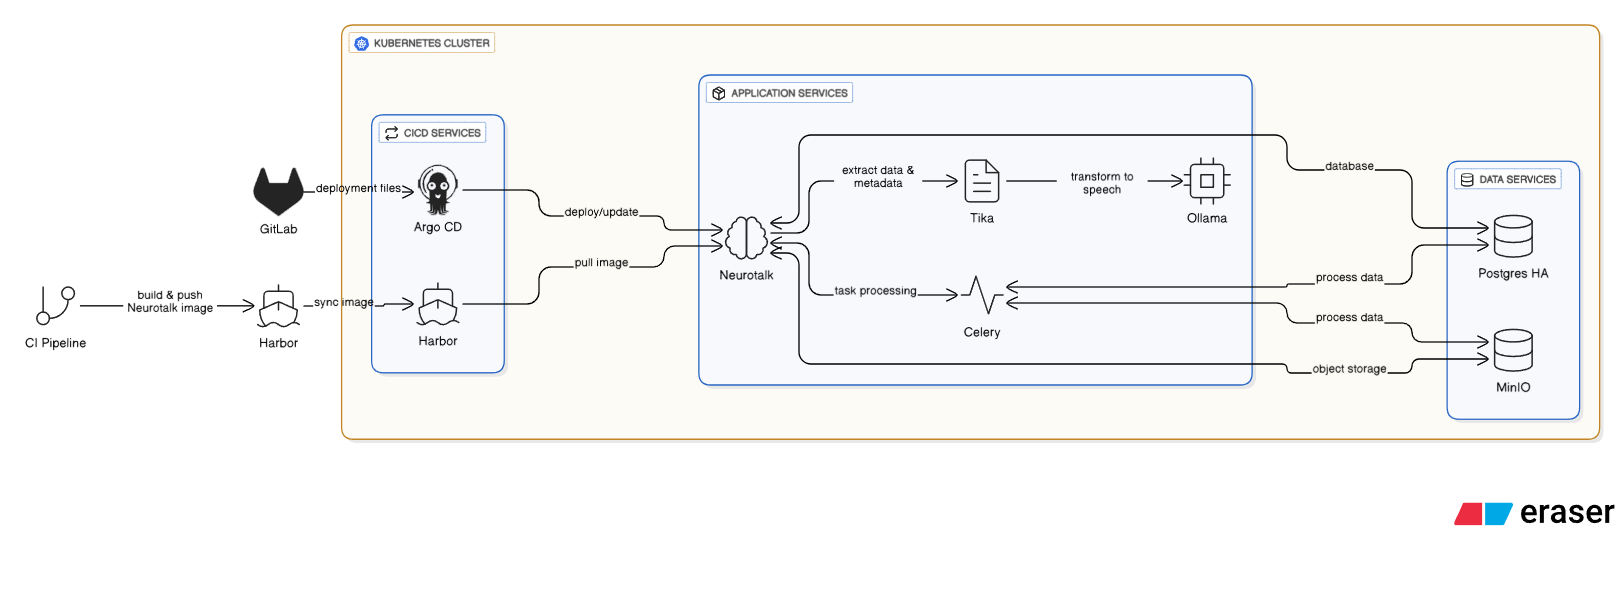
\includegraphics[width=\textwidth]{./assets/NeuroTalk workflow.png}
\caption{NeuroTalk Workflow Diagram}
\end{figure}

Just like with HealthCore, the \textbf{CI Pipeline} builds and pushes the application image to \textbf{Harbor}. \textbf{ArgoCD} then pulls the image and deploys the \textbf{NeuroTalk} application. Once deployed, the application interacts with several other services in the cluster: \textbf{Apache Tika} for document data extraction, \textbf{Ollama} for language processing, and \textbf{Celery} for asynchronous task processing. Data persistence is handled by a \textbf{PostgreSQL HA} (High-Availability) database and \textbf{MinIO} for object storage.

These diagrams effectively illustrate how our platform's design supports a modern, automated, and scalable deployment model for production applications.

\section{Conclusion}
\hspace{1cm}In this chapter, we transitioned from high-level requirements to a concrete architectural design. We used component diagrams to illustrate the logical relationships between our core services and workflow diagrams to detail the automated deployment process for our key applications. This design provides a solid foundation for a resilient and scalable infrastructure.

In the next chapter, we will move on to the practical implementation, detailing the operational procedures for deploying and configuring our Kubernetes cluster.
\end{doublespace}
\newpage

\renewcommand{\headrulewidth}{1pt}
\fancyhead[L]{\textbf{Chapter IV: Implementation}}
\fancyhead[R]{\hspace*{4cm}}

\setcounter{chapter}{4}
\begin{doublespace}
\phantomsection
\addcontentsline{toc}{chapter}{Chapter IV: Implementation}
\vspace*{10cm}
\centering
\textbf{ \huge Chapter IV \\ [1 cm] Implementation}
\end{doublespace}
\setcounter{section}{0}
\newpage

\fancyhead[R]{\nouppercase{\rightmark}}
\begin{doublespace}
 \section*{Introduction}
\hspace{1cm}After completing the analysis and design phase, this chapter focuses on the practical implementation of our work. 
 We begin with a presentation of the main tools and technologies used (software resources, programming languages, frameworks, and supporting tools). 
 Afterwards, we provide details about the features, configurations, and deployment of our high-availability Kubernetes infrastructure and the company services 
 \textbf{NeuroTalk} and \textbf{HealthCore}.
\end{doublespace}

\section{Tools Used}
\begin{doublespace}
\begingroup
\setlength{\parindent}{0pt}

\subsection{Software Resources:}
\noindent%
\\
\begin{minipage}{.7\textwidth}%
\hspace{1cm}\textbf{K3s:} We chose \textbf{K3s}, a lightweight Kubernetes distribution, because it offers the same powerful orchestration capabilities as standard Kubernetes (scaling, self-healing, load balancing) with reduced complexity and resource requirements. 
It is well-suited for production deployments while remaining simple to operate. \\
\textit{How we use it:} We deployed a multi-node K3s cluster that serves as the foundation of our platform, orchestrating \textbf{HealthCore} and \textbf{NeuroTalk} services with high availability and scalability.
\end{minipage}%
\hfill
\begin{minipage}{.2\textwidth}%

\includegraphics[width=\textwidth]{./assets/k3s.png} [2]
\end{minipage} \\ \\ \\

\begin{minipage}{.7\textwidth}%
\hspace{1cm}\textbf{Rancher:} Rancher was selected because it provides a centralized management plane for Kubernetes clusters. It simplifies operations such as cluster provisioning, user management, and monitoring. \\
\textit{How we use it:} We integrated Rancher to manage our K3s cluster with a user-friendly interface, control access rights, and provide administrators with full observability across namespaces and environments.
\end{minipage}%
\hfill
\begin{minipage}{.2\textwidth}%

\includegraphics[width=\textwidth]{./assets/rancher.png} [3]
\end{minipage} \\ \\ \\

\begin{minipage}{.7\textwidth}%
\hspace{1cm}\textbf{ArgoCD:} We adopted ArgoCD for GitOps-based continuous delivery, as it ensures reliable and reproducible deployments. It was chosen for its ability to continuously synchronize the cluster state with Git repositories. \\
\textit{How we use it:} ArgoCD automates deployments for \textbf{HealthCore} and \textbf{NeuroTalk} by pulling Kubernetes manifests and Helm charts from Git, ensuring that the live environment always matches the declared configuration.
\end{minipage}%
\hfill
\begin{minipage}{.2\textwidth}%

\includegraphics[width=\textwidth]{./assets/argocd.png} [4]
\end{minipage} \\ \\ \\

\begin{minipage}{.7\textwidth}%
\hspace{1cm}\textbf{Harbor:} Harbor was chosen as a secure private container registry because it offers image scanning, access control, and integrity verification. \\
\textit{How we use it:} All Docker images built from our CI pipelines are stored in Harbor before deployment. This guarantees trusted and verified images for our Kubernetes workloads.
\end{minipage}%
\hfill
\begin{minipage}{.2\textwidth}%

\includegraphics[width=\textwidth]{./assets/harbor.png} [5]
\end{minipage} \\ \\ \\

\begin{minipage}{.7\textwidth}%
\hspace{1cm}\textbf{NGINX Ingress Controller:} We selected NGINX as the ingress controller due to its robustness, flexibility, and support for advanced routing and SSL termination. \\
\textit{How we use it:} NGINX Ingress routes external traffic to the correct services inside the cluster. For example, requests to \texttt{neurotalk.digitalds.com} and \texttt{healthcore.digitalds.com} are securely routed through it, with certificates handled by Cert-Manager.
\end{minipage}%
\hfill
\begin{minipage}{.2\textwidth}%

\includegraphics[width=\textwidth]{./assets/NGINX.png} [6]
\end{minipage} \\ \\ \\

\begin{minipage}{.7\textwidth}%
\hspace{1cm}\textbf{MinIO:} MinIO was chosen for object storage because it provides S3-compatible APIs in a lightweight and cloud-native form. \\
\textit{How we use it:} Our applications rely on MinIO to store medical reports, documents, and unstructured datasets. It is deployed in distributed mode to ensure durability and scalability.
\end{minipage}%
\hfill
\begin{minipage}{.2\textwidth}%

\includegraphics[width=\textwidth]{./assets/minio.png} [7]
\end{minipage} \\ \\ \\

\begin{minipage}{.7\textwidth}%
\hspace{1cm}\textbf{PostgreSQL HA:} PostgreSQL was selected as the primary relational database because of its reliability, scalability, and advanced SQL support. We configured it in High-Availability mode to avoid downtime. \\
\textit{How we use it:} PostgreSQL stores structured data for \textbf{HealthCore} and \textbf{NeuroTalk}. It runs as a StatefulSet with persistent volumes, and is paired with \textbf{PgBouncer} for efficient connection pooling.
\end{minipage}%
\hfill
\begin{minipage}{.2\textwidth}%
\includegraphics[width=\textwidth]{./assets/postgresql.png} [8]
\end{minipage} \\ \\ \\


\subsection{Programming Languages:}
\noindent%
\\
\begin{minipage}{.76\textwidth}%
\hspace{1cm}\textbf{YAML:} Chosen for its readability and simplicity, YAML is the standard for defining Kubernetes resources. \\
\textit{How we use it:} All deployments, services, ingress rules, and persistent volume claims are defined as YAML manifests and version-controlled in Git.
\end{minipage}%
\hfill
\begin{minipage}{.2\textwidth}%

\includegraphics[width=\textwidth]{./assets/yaml.jpg} [9]
\end{minipage} \\ \\ \\

\begin{minipage}{.76\textwidth}%
\hspace{1cm}\textbf{Bash:} Bash was chosen for automation tasks because it is lightweight and ubiquitous across systems. \\
\textit{How we use it:} Bash scripts automate cluster bootstrapping, application deployments, and CI/CD tasks for reproducibility.
\end{minipage}%
\hfill
\begin{minipage}{.2\textwidth}%

\includegraphics[width=\textwidth]{./assets/bash.png} [10]
\end{minipage} \\

\subsection{Supporting Tools:}
\noindent%
\\
\begin{minipage}{.76\textwidth}%
\hspace{1cm}\textbf{Helm:} We selected Helm because it simplifies the deployment of complex applications with reusable charts. \\
\textit{How we use it:} PostgreSQL HA, Harbor, and MinIO were deployed using official Helm charts, reducing manual configuration and ensuring consistent deployments.
\end{minipage}%
\hfill
\begin{minipage}{.2\textwidth}%

\includegraphics[width=\textwidth]{./assets/helm.png} [11]
\end{minipage} \\ \\ \\

\endgroup
\end{doublespace}

\newpage

\section{Set up and Configuration}
\begin{doublespace}

\subsection{Cluster Dashboard (Rancher)}
\hspace{1cm}The platform runs on a K3s cluster managed via Rancher. The cluster dashboard provides an overview of resources (pods, CPU, memory) and the general health of the environment, which is essential for capacity planning and SRE operations.
\begin{figure}[H]
\centering
  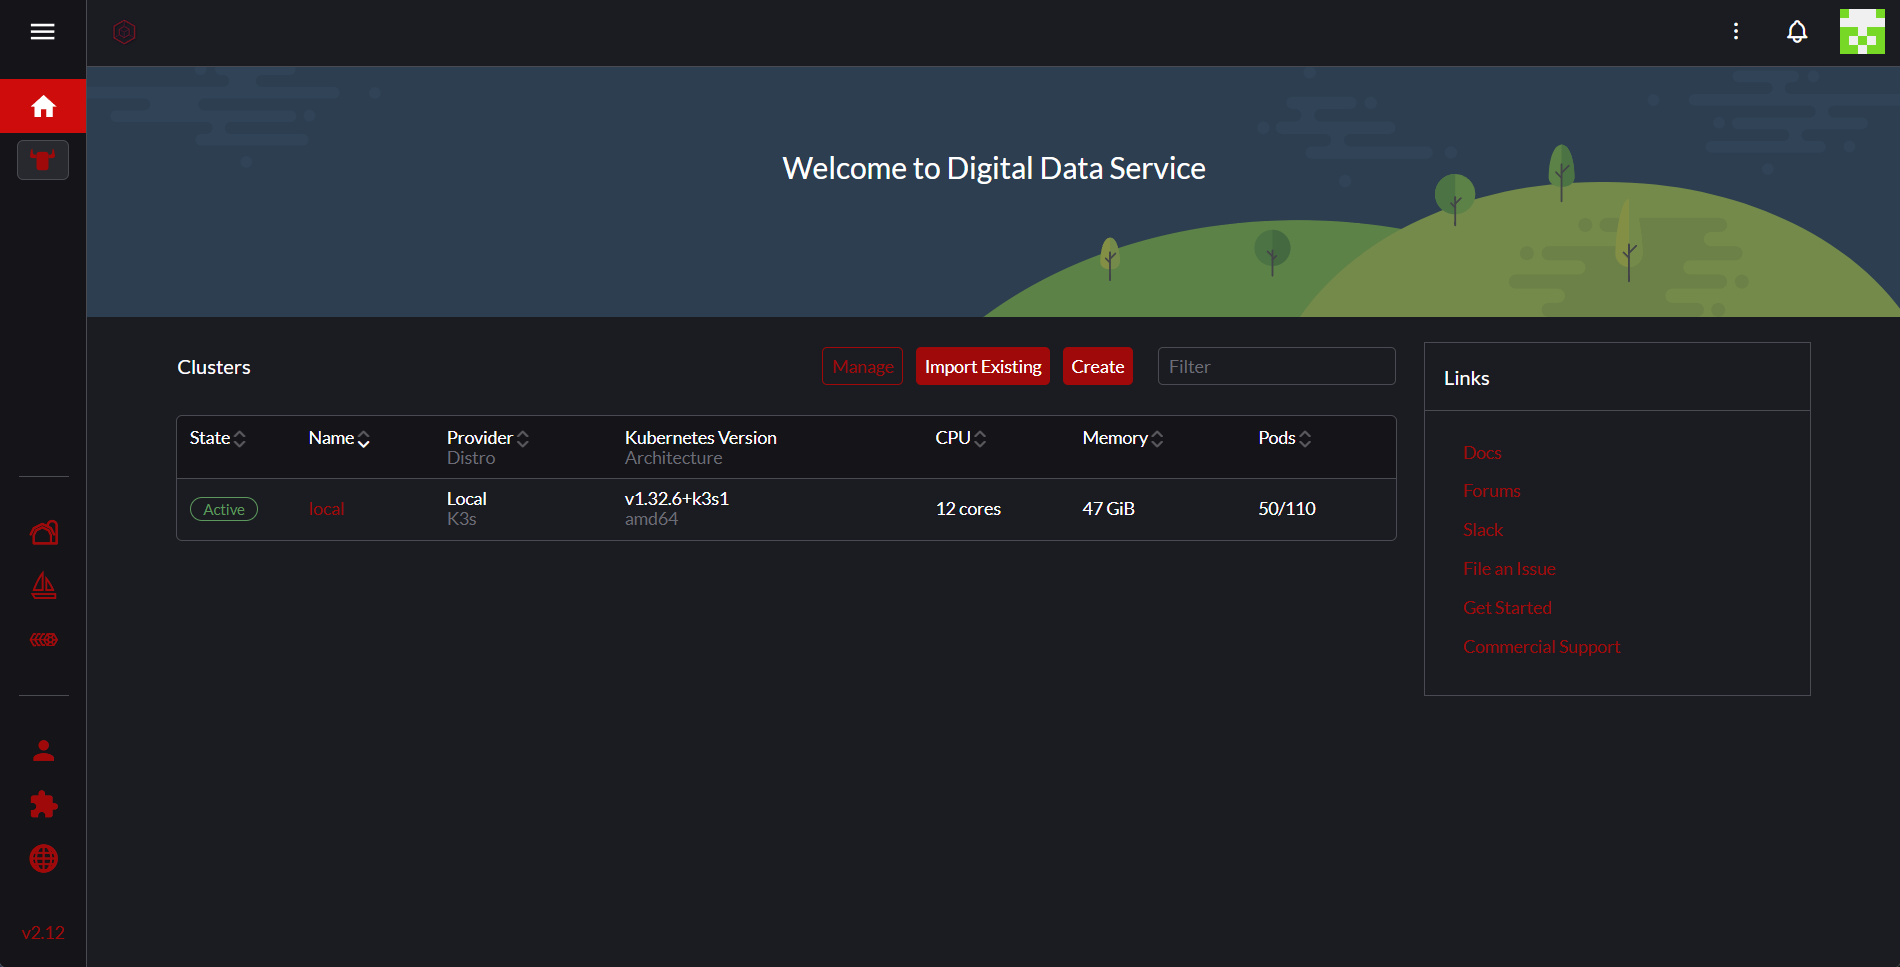
\includegraphics[width=\textwidth]{assets/Screenshot 2025-08-22 144839.png}
\caption{Rancher cluster dashboard overview}
\end{figure}

\subsection{Projects and Namespaces}
\hspace{1cm}Rancher’s Projects/Namespaces view is used to segment workloads (e.g., harbor, minio, postgres, redis, tika, neurotalk) and system components (e.g., cnpg-system). This enforces isolation, RBAC scoping, and resource quotas per team or service.
\begin{figure}[H]
\centering
  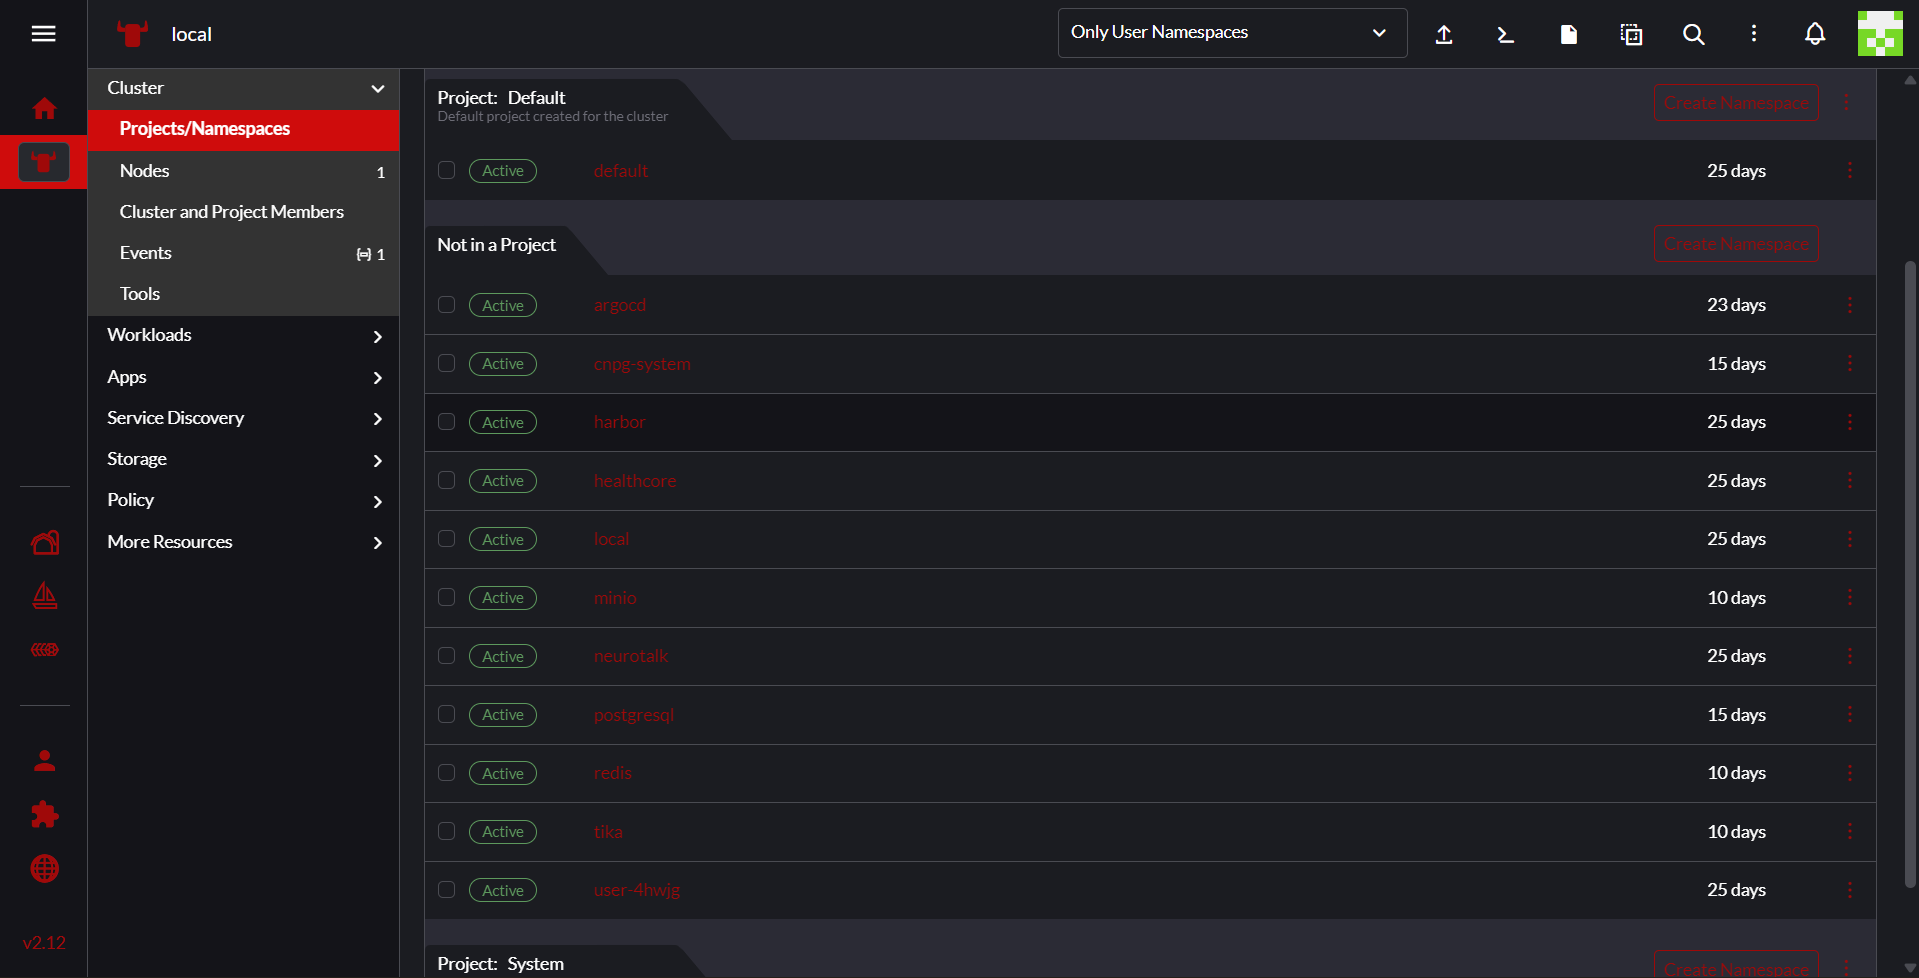
\includegraphics[width=\textwidth]{assets/Screenshot 2025-08-22 144917.png}

\caption{Logical isolation via Projects/Namespaces}
\end{figure}

\subsection{Container Registry (Harbor)}
\hspace{1cm}Harbor hosts our private OCI images, organized by projects (e.g., healthcare, neurotalk-front, neurotalk-back, library). It provides vulnerability scanning, role-based access, and image retention policies to keep the registry clean and secure.
\begin{figure}[H]
\centering
  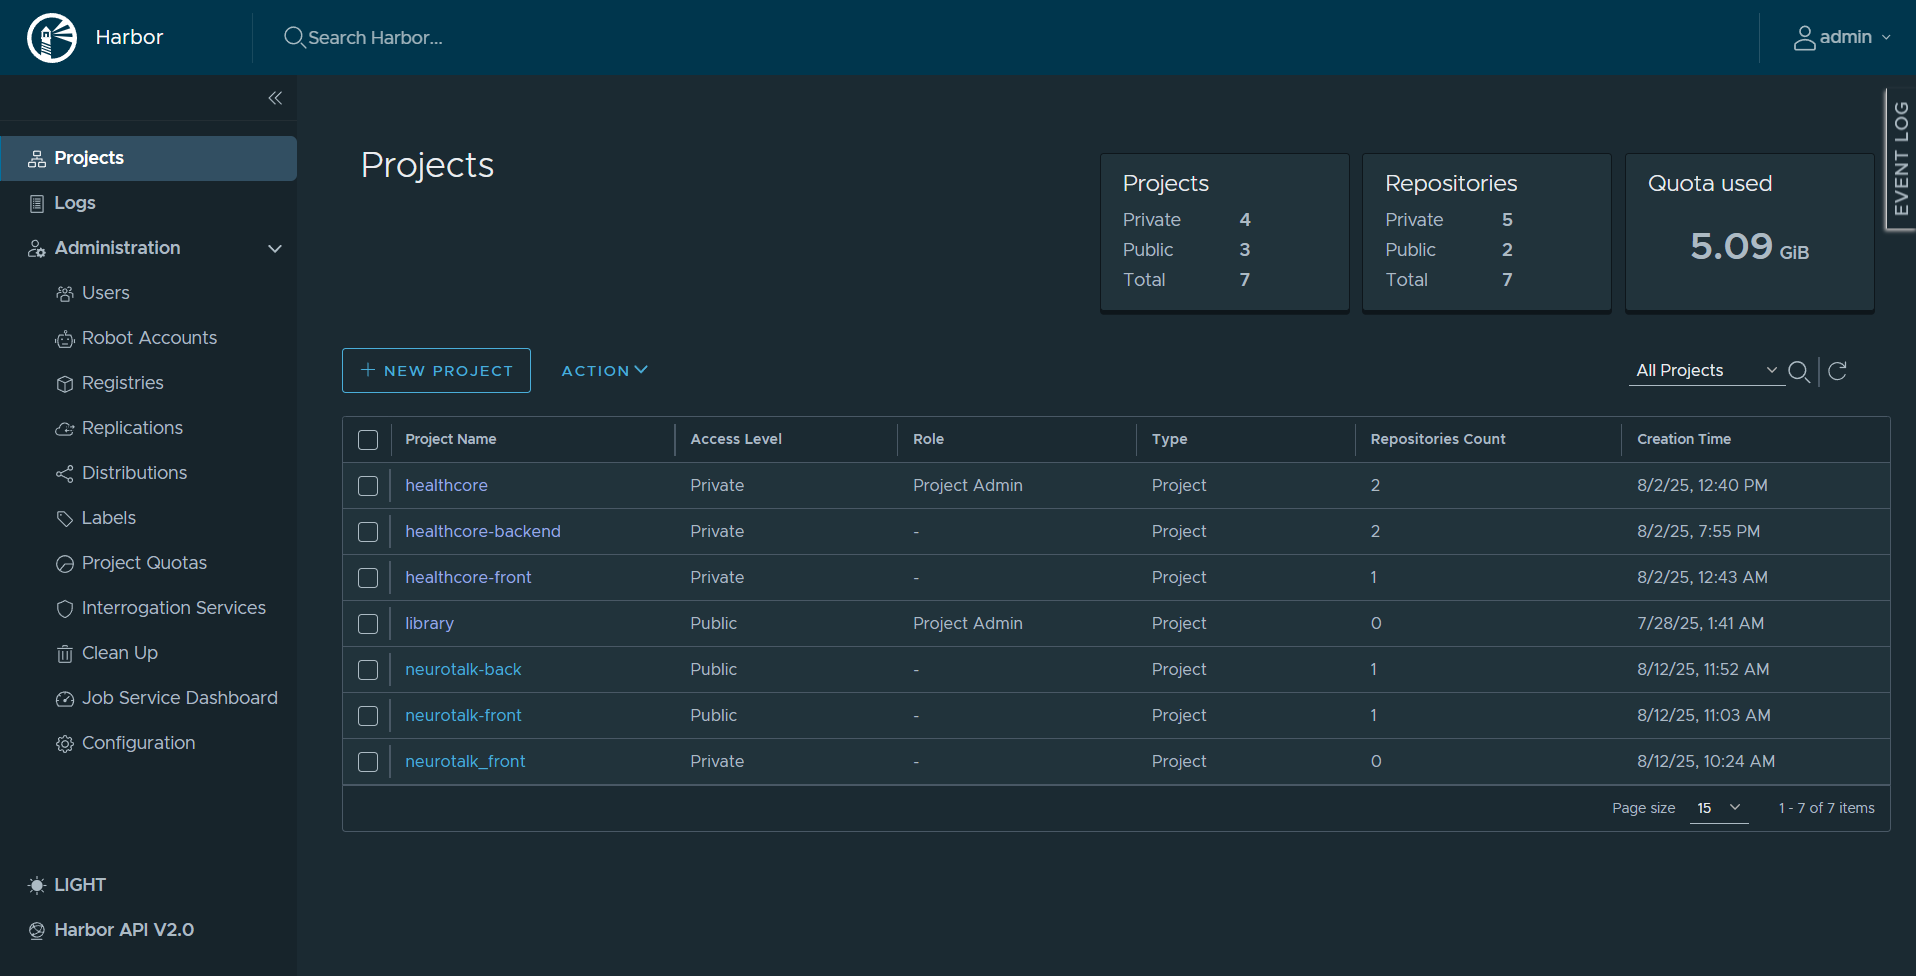
\includegraphics[width=\textwidth]{assets/Screenshot 2025-08-22 144941.png}
\caption{Harbor projects used for image management}
\end{figure}

\subsection{GitOps Dashboard (Argo CD)}
\hspace{1cm}Deployments are managed with GitOps using Argo CD. Each \textit{Application} tracks a Git repository, path, and target revision, and continuously reconciles the live cluster state with the desired state from Git. Argo CD exposes two key signals: \textbf{Health} (e.g., Healthy/Degraded) and \textbf{Sync} (Synced/OutOfSync).

\begin{itemize}
  \item Applications: \texttt{healthcore-backend} and \texttt{healthcore-frontend}
  \item Destination: \texttt{in-cluster} \quad Namespace: \texttt{healthcore} \quad Project: \texttt{default}
  \item Repos/Paths: Git (GitLab), paths \texttt{k8s/base/backend} and \texttt{k8s/base/frontend}
  \item Status (from snapshot): both \textbf{Healthy}; frontend \textbf{Synced}, backend \textbf{Synced}
\end{itemize}\begin{figure}[H]
\centering
  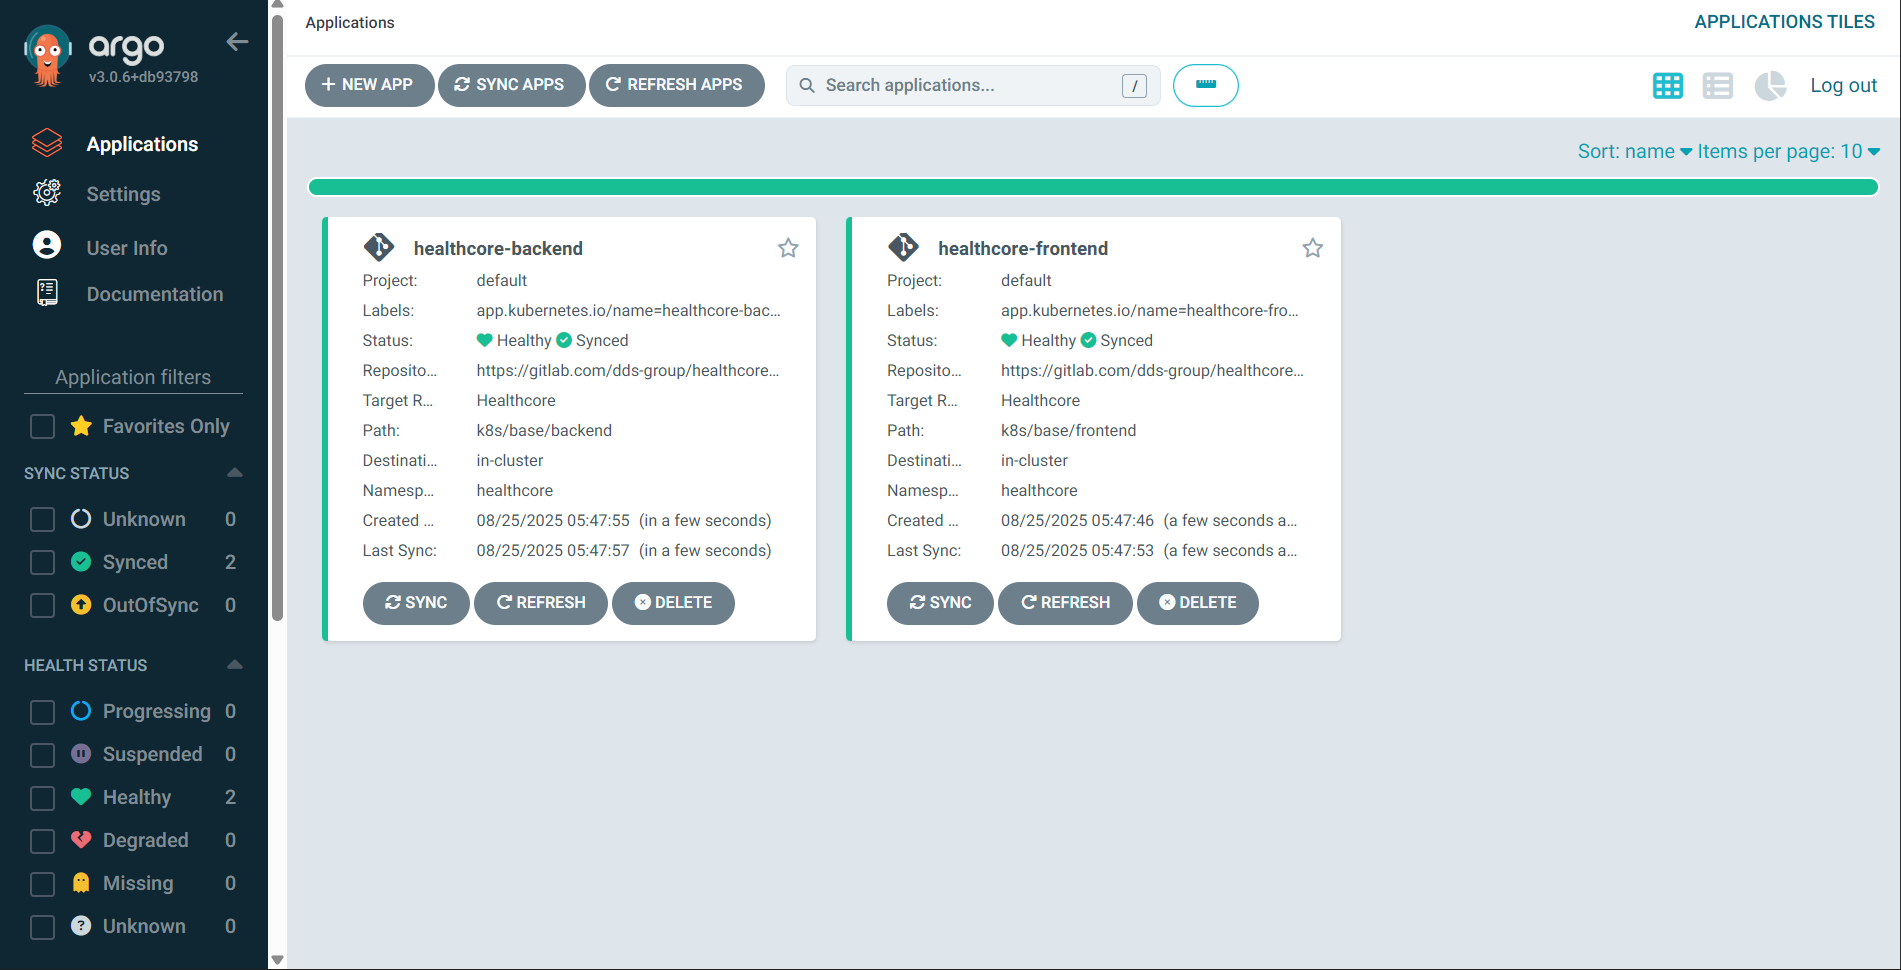
\includegraphics[width=\textwidth]{assets/Screenshot 2025-08-25 054803.png}
\caption{Argocd Overview}
\end{figure}

\subsection{Object Storage (MinIO)}
\hspace{1cm}MinIO provides S3-compatible object storage used for application assets, backups, and model artifacts. Buckets and policies are managed through the MinIO Console.
\begin{figure}[H]
\centering
  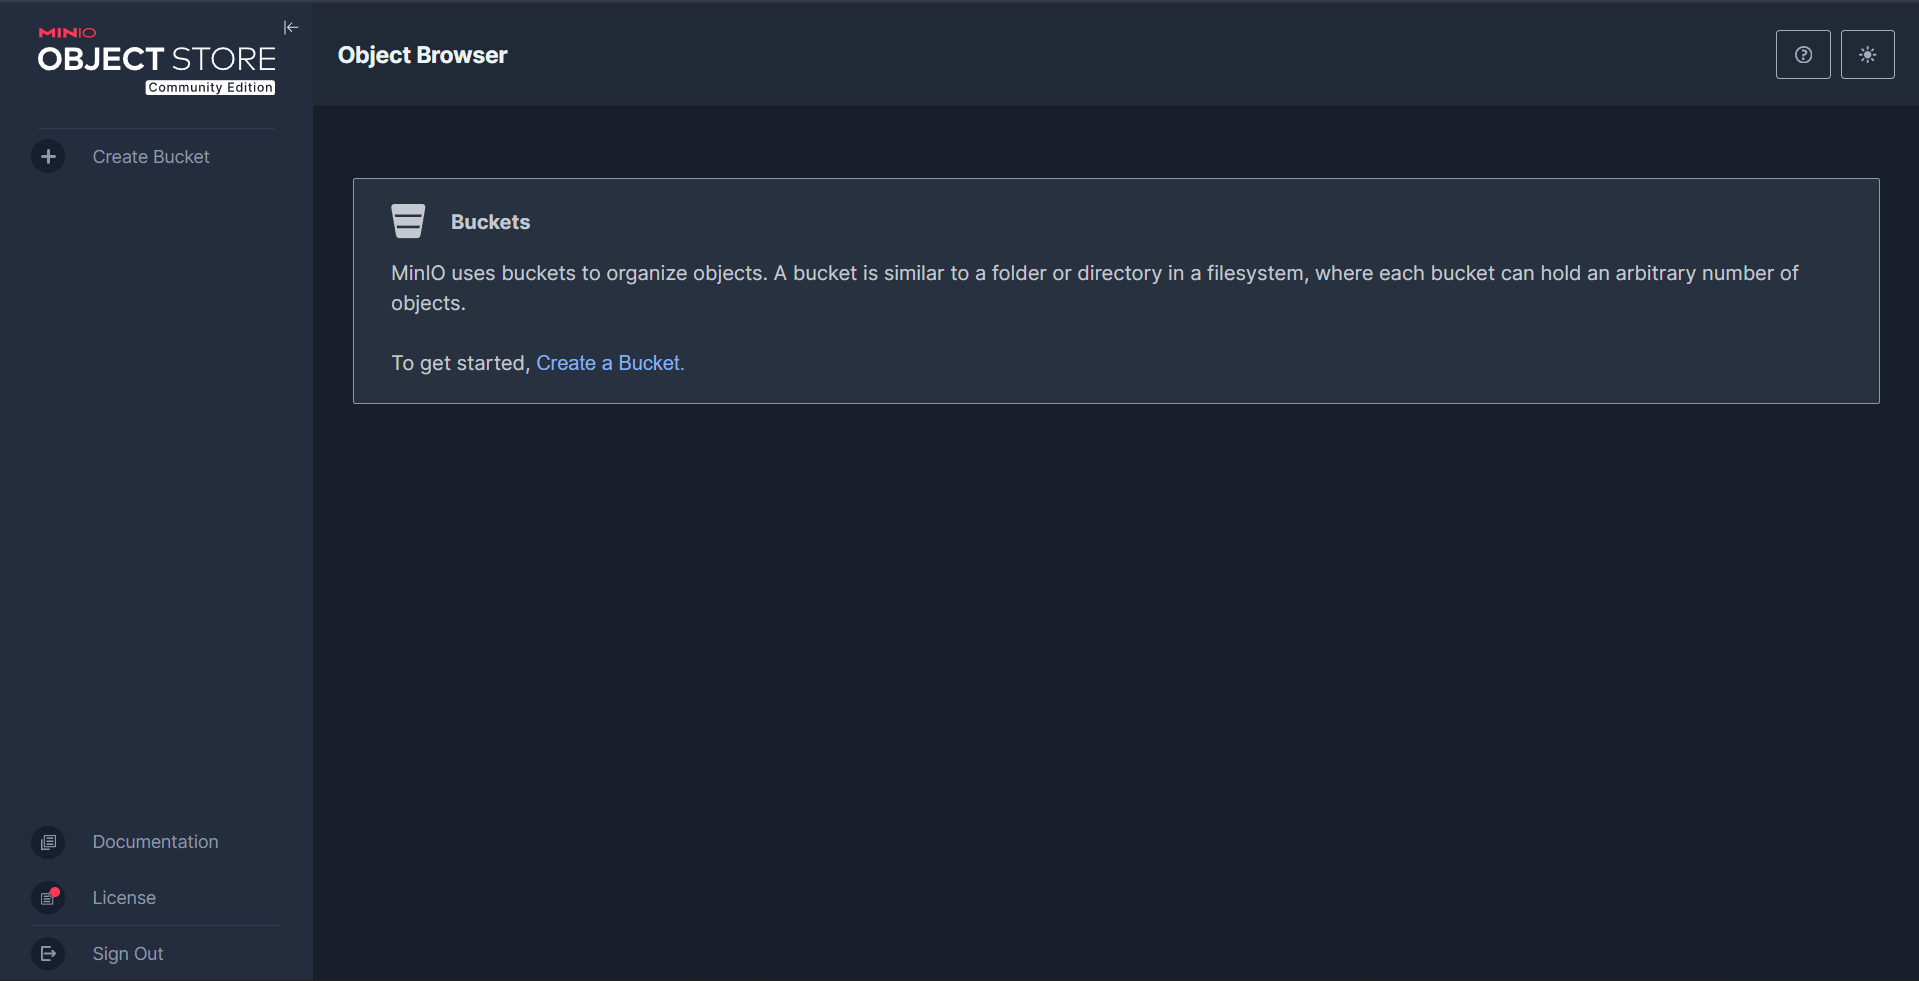
\includegraphics[width=\textwidth]{assets/Screenshot 2025-08-22 145019.png}
\caption{MinIO Object Store Console}
\end{figure}

\subsection{Relational Database (PostgreSQL)}
\hspace{1cm}PostgreSQL backs transactional data. Administration is performed through pgAdmin for observability and maintenance (roles, schemas, backups). In production, we rely on Kubernetes-native HA patterns (e.g., CloudNativePG or replicated StatefulSets) with persistent volumes.
\begin{figure}[H]
\centering
  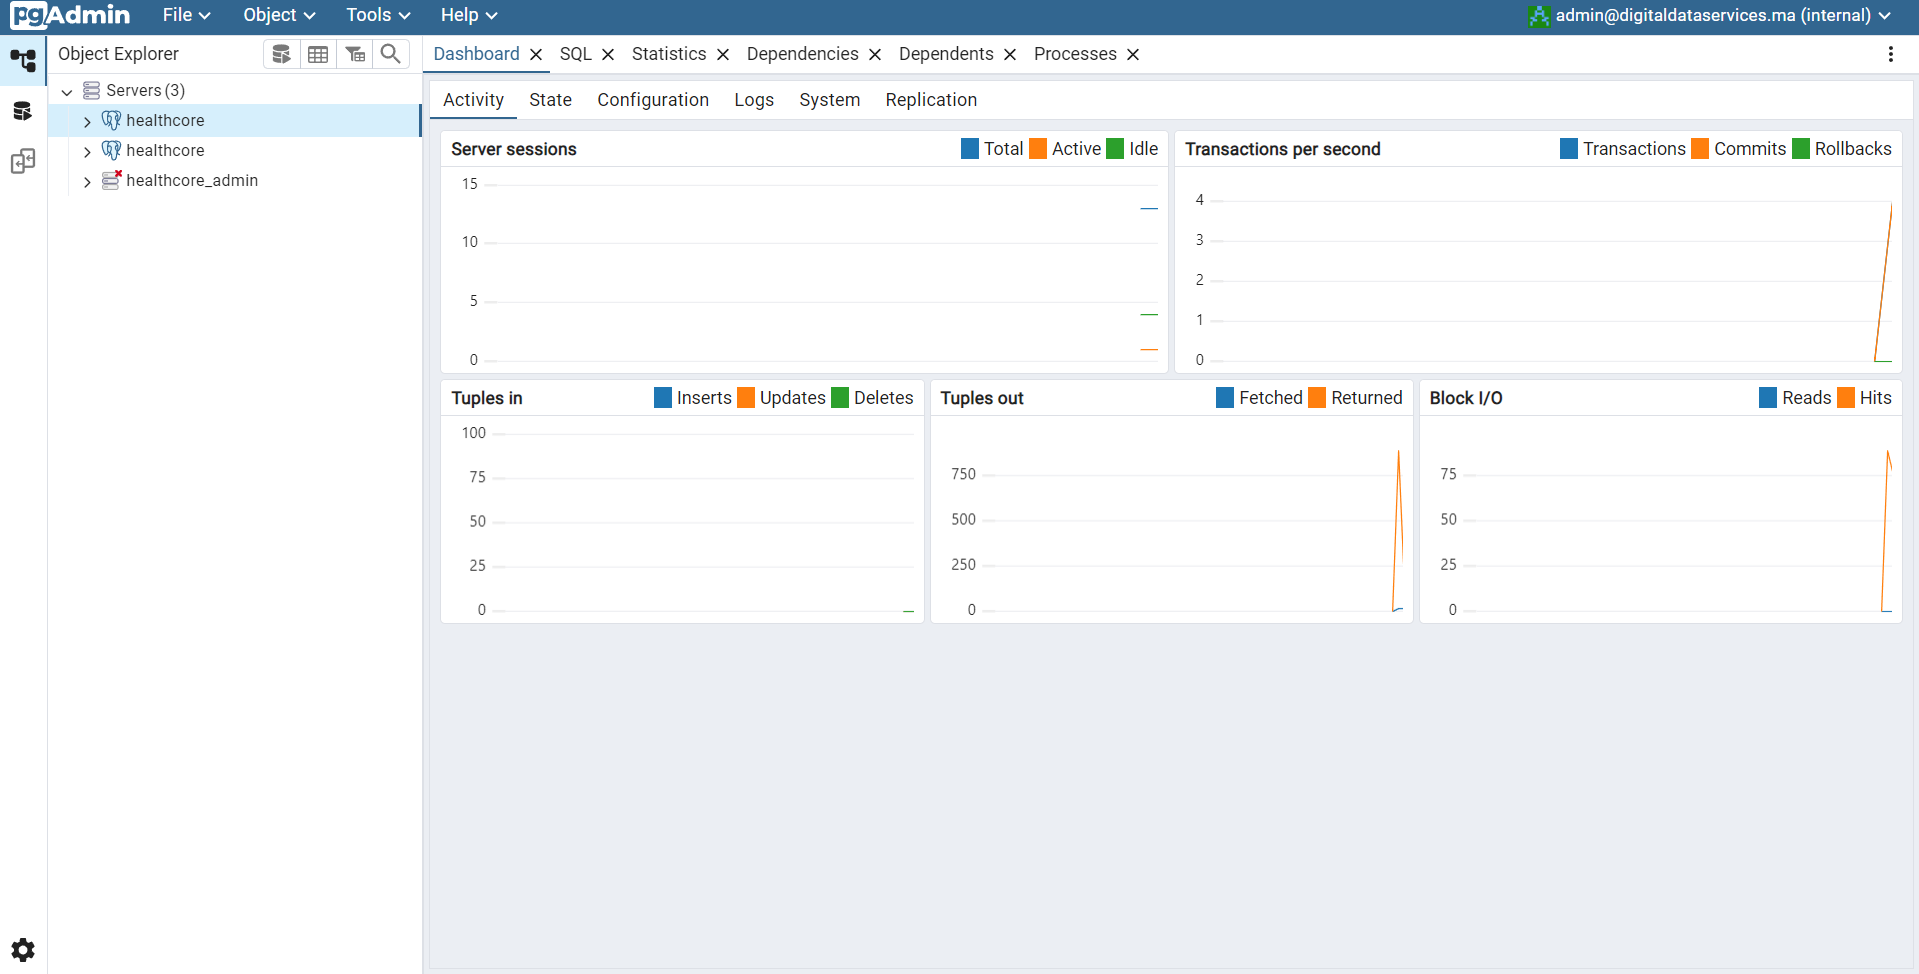
\includegraphics[width=\textwidth]{assets/Screenshot 2025-08-22 145152.png}
\caption{pgAdmin attached to the PostgreSQL cluster}
\end{figure}

\subsection{Persistent Volumes (PVCs)}
\hspace{1cm}Stateful components (Harbor, PostgreSQL, Redis, MinIO) use PersistentVolumeClaims (PVCs) backed by the local-path storage class in this environment. The kubectl view confirms all critical PVCs are Bound with the expected capacity and access mode.
\begin{figure}[H]
\centering
  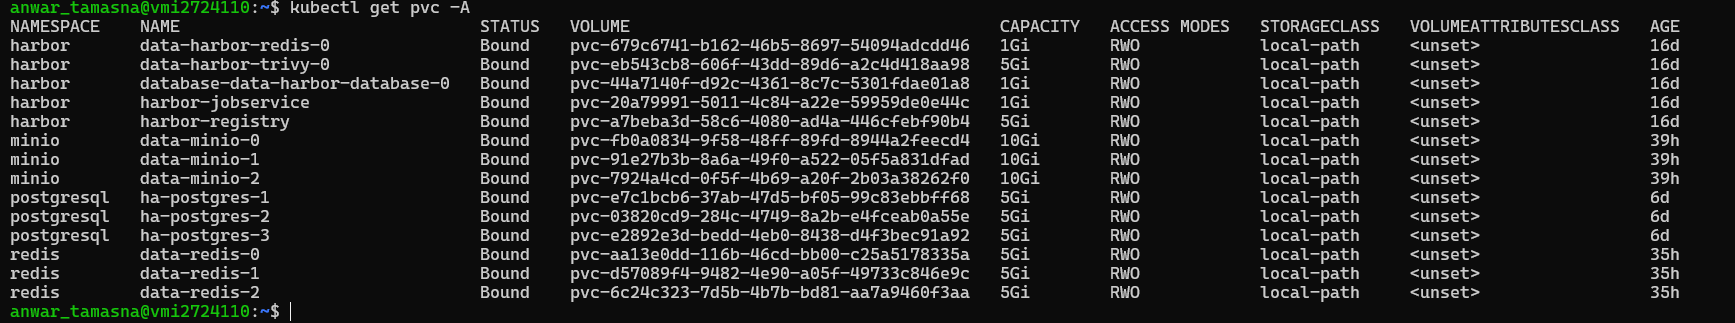
\includegraphics[width=\textwidth]{assets/Screenshot 2025-08-13 144018.png}
\caption{Cluster-wide PVC status for stateful workloads}
\end{figure}

\subsection{Workload Layout (NeuroTalk stack)}
\hspace{1cm}NeuroTalk components are organized as separate services: API, Celery workers, Redis for caching/queues, Tika for document processing, and Ollama for local LLM inference. This layout simplifies CI/CD and operational boundaries.
\begin{figure}[H]
\centering
  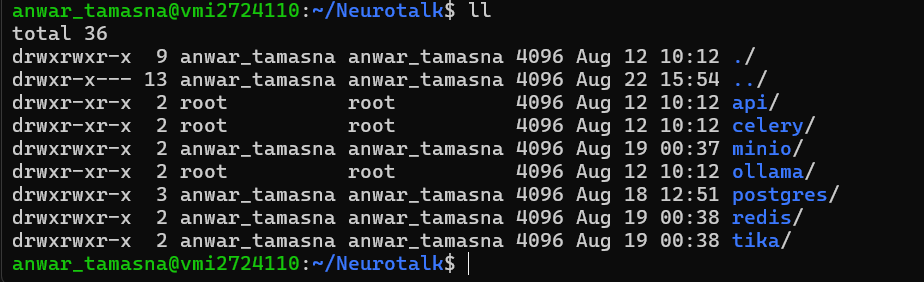
\includegraphics[width=\textwidth]{assets/Screenshot 2025-08-22 145703.png}
\caption{NeuroTalk stack directory structure}
\end{figure}

\subsection{MinIO Kubernetes Manifests}
\hspace{1cm}The MinIO deployment is defined via manifests (Deployment/StatefulSet, Secret, Ingress). Secrets store access and console credentials; the Ingress exposes the console/API over HTTPS (behind the cluster ingress controller).
\begin{figure}[H]
\centering
  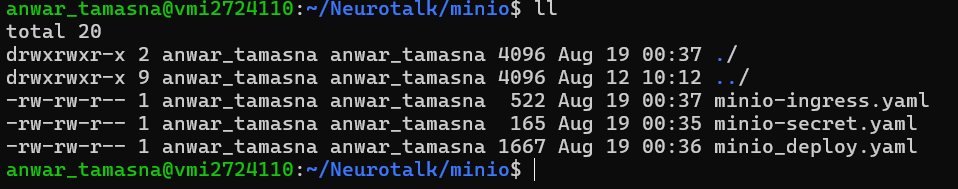
\includegraphics[width=\textwidth]{assets/Screenshot 2025-08-22 145730.png}
\caption{MinIO Kubernetes manifests}
\end{figure}

\subsection{PostgreSQL and pgAdmin Manifests}
\hspace{1cm}PostgreSQL and pgAdmin are deployed via manifests that define storage (PVCs), services, and optional Ingress. For HA and operational automation, CloudNativePG or similar operators can be used to manage upgrades and failover.
\begin{figure}[H]
\centering
  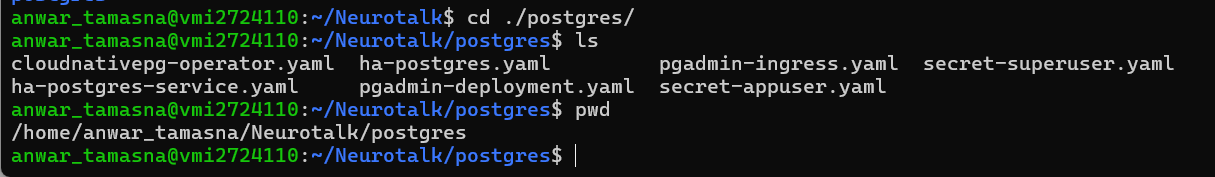
\includegraphics[width=\textwidth]{assets/Screenshot 2025-08-11 213050.png}
\caption{PostgreSQL and pgAdmin deployment resources}
\end{figure}

\subsection{Security and Operations Highlights}
\hspace{1cm}We enforce RBAC at the namespace/project level, use private images from Harbor, and store credentials in Kubernetes Secrets. Persistent volumes are provisioned per stateful service. Monitoring/alerting is integrated via the cluster stack, and backups are stored on MinIO with lifecycle policies.

\end{doublespace}


\section{Benchmark}
\begin{doublespace}
\hspace{1cm}This snapshot comes from the Rancher Cluster Dashboard and summarizes current capacity and health. It provides a fast read on performance headroom for the Kubernetes platform.

\subsection*{Environment}
\hspace{1cm}K3s \textbf{v1.32.6+k3s1} (amd64), cluster age \textbf{25 days}, \textbf{1} node, \textbf{31} deployments, \textbf{386} total resources.

\begin{figure}[H]
\centering
  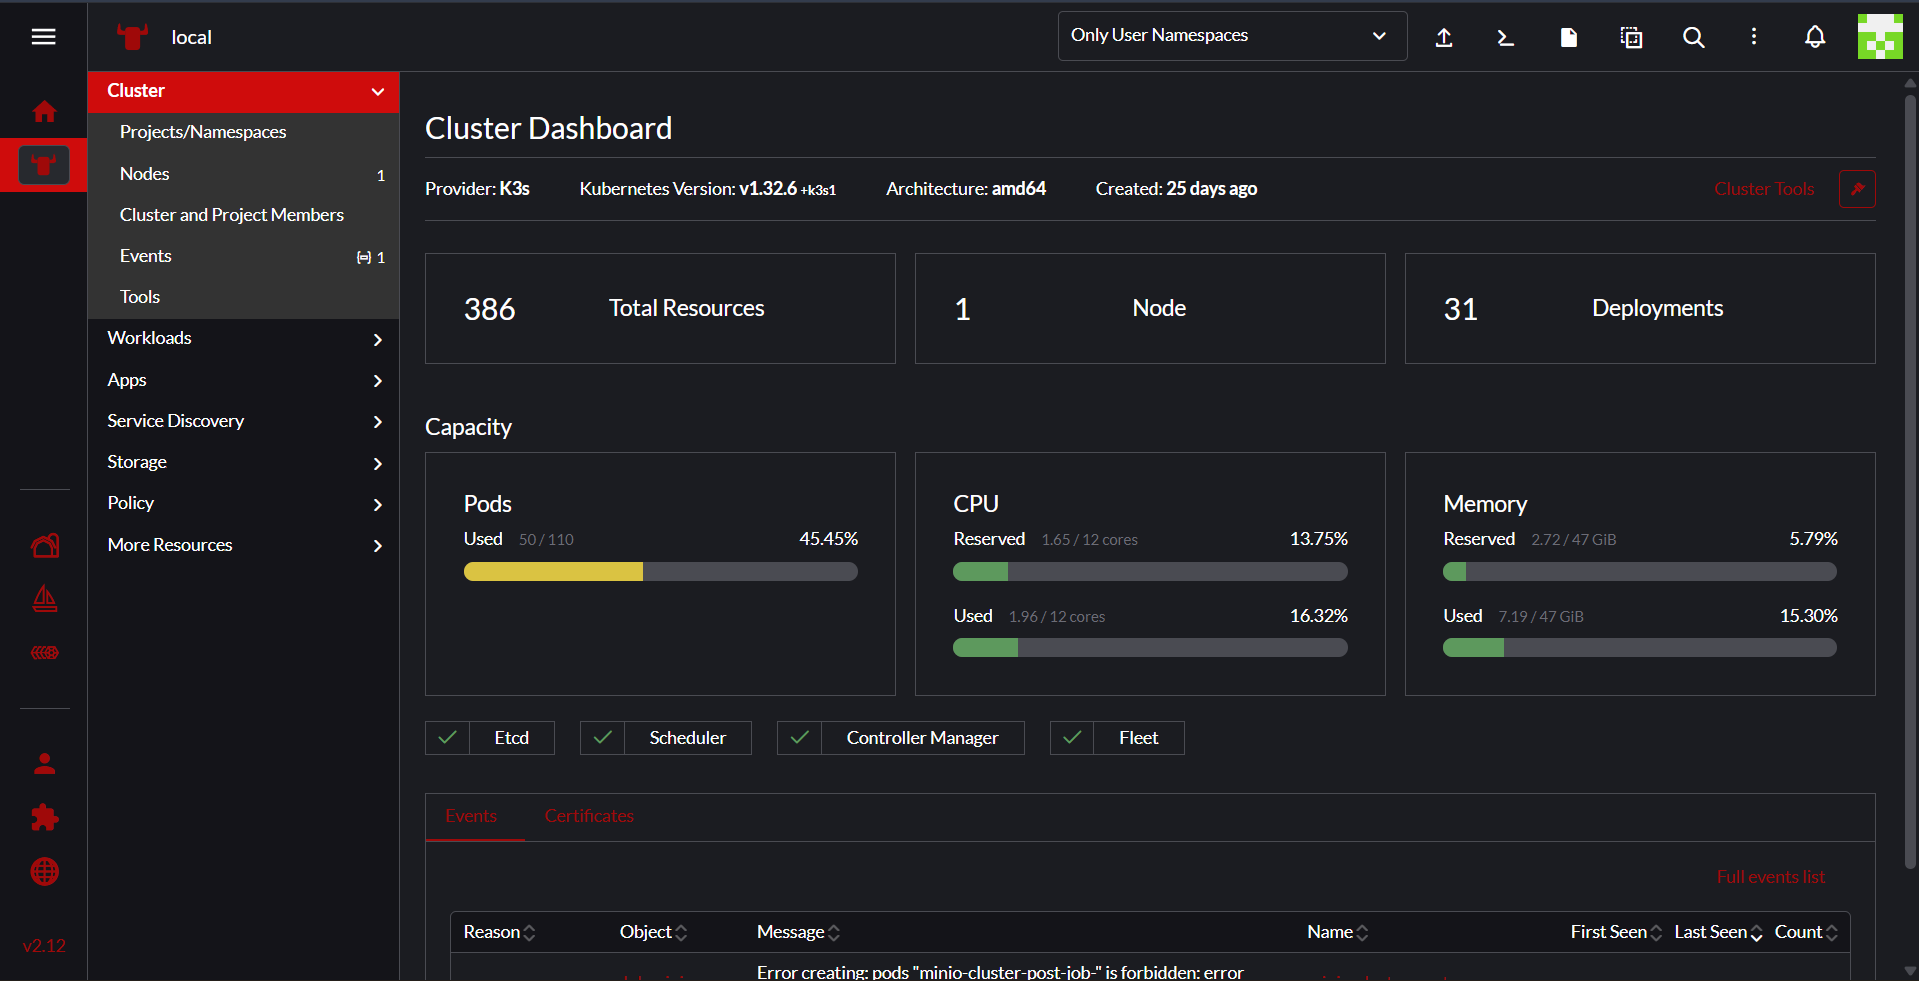
\includegraphics[width=\textwidth]{assets/Screenshot 2025-08-22 144903.png}
\caption{Cluster dashboard snapshot (Rancher)}
\end{figure}

\subsection*{Instant Utilization}
\begin{itemize}
  \item Pods: \textbf{50 / 110} (\textbf{45.45\%})
  \item CPU: reserved \textbf{1.65 / 12} (\textbf{13.75\%}); used \textbf{1.96 / 12} (\textbf{16.32\%})
  \item Memory: reserved \textbf{2.72 / 47 GiB} (\textbf{5.79\%}); used \textbf{7.19 / 47 GiB} (\textbf{15.30\%})
  \item Control plane: Etcd, Scheduler, Controller Manager, Fleet — \textbf{healthy}
\end{itemize}

\subsection*{Performance Interpretation}
\begin{itemize}
  \item Low CPU (\textasciitilde16\%) and memory (\textasciitilde15\%) usage indicate ample headroom; short spikes and moderate scale-outs will not contend for resources on this node.
  \item Pod usage at 45\% (50/110) leaves capacity for \textasciitilde60 additional pods, assuming similar resource profiles.
  \item Reserved vs. used shows minimal overcommit (13.75\% reserved), so current quotas/limits are conservative and safe.
  \item Control-plane components are green, suggesting stable scheduling, persistence, and cluster state.
\end{itemize}

\subsection*{Quick Requirements Check}
\begin{itemize}
  \item Health budget: core services healthy — \textbf{Pass}
  \item Headroom: CPU, memory, pods all $<$ 50\% — \textbf{Pass}
  \item Overcommit: reserved CPU/memory $<$ 25\% — \textbf{Pass}
\end{itemize}

\section{Conclusion}
\hspace{1cm}In summary, the Rancher Cluster Dashboard provides a comprehensive overview of the current state of the Kubernetes environment. The utilization metrics indicate that the cluster is operating well within its capacity limits, with ample headroom for future growth. The deployment strategies for key components like NeuroTalk, MinIO, PostgreSQL, and pgAdmin are well-defined, leveraging Kubernetes best practices for security, scalability, and maintainability. Overall, the cluster is in a healthy state, ready to support the demands of the applications it hosts.
\end{doublespace}


\phantomsection
\addcontentsline{toc}{section}{General Conclusion}
\begin{center}
\vspace{9cm}
    \textbf{\huge{General Conclusion}}
\end{center}

\renewcommand{\headrulewidth}{1pt}
\fancyhead[R]{\textbf{General Conclusion}}
\fancyhead[L]{\hspace*{4cm}}

\begin{doublespace}
I am very pleased to have completed my internship at \textbf{Digital Data Service}, where I contributed to the development and deployment of innovative solutions with a strong focus on \textbf{Kubernetes (K3s)}, containerization, and modern DevOps practices. This experience allowed me to gain a deeper understanding of the technical and organizational challenges of building scalable, reliable, and secure infrastructures for digital platforms.\\

From a technical standpoint, the project delivered a cohesive, production-like platform that unifies cluster management, secure image delivery, persistence, and automated deployments. Key outcomes:\\
\begin{itemize}
    \item \textbf{K3s + Rancher}: centralized cluster ops with namespaces and RBAC.
    \item \textbf{GitOps with ArgoCD}: declarative, auditable, and reproducible releases.
    \item \textbf{NGINX Ingress + Cert-Manager}: secure exposure with automated TLS.
    \item \textbf{Harbor + persistence}: private registry; MinIO, PostgreSQL HA, Redis, Tika where needed.
    \item \textbf{App staging}: NeuroTalk and HealthCore validated with persistent data and env configs.
\end{itemize}

Lessons learned:
\begin{itemize}
    \item Favor \textbf{declarative} config and version control for all infra artifacts.
    \item Build \textbf{observability} early (metrics, logs, alerts) to shorten feedback loops.
\end{itemize}

Constraints and mitigations:
\begin{itemize}
    \item Time and hardware limited scope; used local-path storage pragmatically.
    \item Drift curbed by \textbf{GitOps}; rollback safety via versioned releases/immutable images.
    \item Stateful reliability via PVCs, health probes, and periodic backups.
\end{itemize}

Next steps (roadmap):
\begin{itemize}
    \item Expand monitoring (\textbf{Prometheus, Grafana, Loki}) and SLO-based alerting.
    \item Strengthen security (OPA/Gatekeeper, Cosign, External Secrets + Vault).
    \item Improve \textbf{backup/DR} with Velero and tested runbooks.
    \item Add autoscaling on custom metrics and safer rollouts (blue/green, canary).
    \item Explore multi-zone and multi-node control planes; enforce NetworkPolicies.
\end{itemize}

In conclusion, the platform establishes a solid, scalable foundation. With incremental investments in monitoring, security, and resilience, it is well positioned to operate reliably at production scale.
\end{doublespace}

\renewcommand{\headrulewidth}{1pt}
\fancyhead[R]{\textbf{General Conclusion}}
\fancyhead[L]{\hspace*{4cm}}

\newpage
\renewcommand{\headrulewidth}{1pt}
\fancyhead[R]{\textbf{BIBLIOGRAPHY}}
\fancyhead[L]{\hspace*{4cm}}
\begin{center}
\textbf{\huge{BIBLIOGRAPHY}}

\end{center}
\begin{doublespace}
\large{
\begin{enumerate}
    \item Digital Data Service — Technical fact sheet (PDF). Internal document.
    \item K3s image. \url{https://docs.k3s.io/}. Accessed: 22-08-25.
    \item Rancher brand guidelines (logo). \url{https://www.rancher.com/brand-guidelines}. Accessed: 22-08-25.
    \item Argo CD image. \url{https://gitlab.com/gitlab-com/gl-infra/k8s-workloads/argocd}. Accessed: 22-08-25.
    \item Harbor logo. \url{https://seeklogo.com/vector-logo/447018/harbor}. Accessed: 22-08-25.
    \item NGINX icon. \url{https://techicons.dev/icons/nginx}. Accessed: 22-08-25.
    \item MinIO compliance (logo). \url{https://www.min.io/compliance}. Accessed: 22-08-25.
    \item PostgreSQL logo. \url{https://commons.wikimedia.org/wiki/File:Postgresql_elephant.svg}. Accessed: 22-08-25.
    \item YAML file icon. \url{https://fr.pngtree.com/freepng/yaml-file-document-icon_4177017.html}. Accessed: 22-08-25.
    \item Bash logo. \url{https://bashlogo.com/}. Accessed: 22-08-25.
    \item Helm logo. \url{https://www.pngegg.com/en/png-vensc}. Accessed: 22-08-25.
\end{enumerate}
}
\end{doublespace}
\end{document}

